% =========================================================================
% SUMÁRIO (ANTES DO RESUMO)
% =========================================================================
\pagestyle{empty}
\renewcommand{\contentsname}{Sumário}
\setcounter{tocdepth}{1}
\tableofcontents
\clearpage

% =========================================================================
% RESUMO E INTRODUÇÃO (COMPARTILHAM UMA ÚNICA PÁGINA)
% =========================================================================
\pagestyle{textual}
% =========================================================================
% SEÇÃO 1: RESUMO
% =========================================================================
\section{Resumo}\label{sec:resumo}

Fluxos em digrafos constituem uma área fundamental da Otimização Combinatória, com amplas aplicações práticas em redes de transporte e alocação de recursos. Este projeto adota uma abordagem que combina fundamentos teóricos, implementação algorítmica e validação experimental para o estudo de problemas de fluxo máximo e fluxo de custo mínimo (veja~\cite{ahuja1993network}). Foram estudados e implementados algoritmos clássicos e modernos de fluxo máximo e de fluxo de custo mínimo, bem como técnicas de modelagem e reduções combinatórias, incluindo a aplicação prática em Segmentação Interativa de Imagens via corte mínimo. A validação prática foi realizada através de experimentos computacionais utilizando instâncias de \textit{benchmarks} reconhecidas da literatura (veja~\cite{Jensen2022}).


\vspace{0.35cm}

% =========================================================================
% SEÇÃO 2: INTRODUÇÃO
% =========================================================================
\section{Introdução}\label{sec:introducao}

A Otimização Combinatória é uma área de pesquisa situada na interseção entre Matemática e Ciência da Computação (veja~\cite{korte2018combinatorial}). Do ponto de vista matemático, a área mantém forte influência com a Teoria dos Grafos, uma vez que digrafos constituem objetos combinatórios com amplo poder de modelagem (veja~\cite{bondy2008graph, diestel2017graph}).
Sob a perspectiva computacional, o foco reside na obtenção de algoritmos eficientes que produzam soluções garantidamente ótimas (veja~\cite{schrijver2003combinatorial, cook1998combinatorial}). Dentre os tópicos de destaque, os problemas de fluxos em digrafos ocupam posição central, tratando de redes onde recursos devem ser transportados respeitando restrições de capacidade (veja~\cite{ahuja1993network}).
O objetivo deste projeto é proporcionar uma formação sólida na área, integrando teoria e prática, abrangendo desde fundamentos conceituais até implementações de alta performance em C++23 e aplicações reais em Visão Computacional.

O problema do $st$-fluxo máximo, onde se busca maximizar a quantidade de fluxo enviada de um vértice fonte $s$ para um vértice de destino $t$, é um dos pilares deste estudo (veja~\cite{ford1956maximal}). Foram analisados e implementados algoritmos clássicos e eficientes, como Ford-Fulkerson, Edmonds-Karp, Dinic e Push-Relabel com Heurística de Gap (veja~\cite{ford1956maximal, edmonds1972theoretical, dinic1970algorithm, goldberg1988new}).
O projeto contempla também o problema de fluxo de custo mínimo, que busca minimizar o custo total enquanto satisfaz as demandas da rede, com destaque para os algoritmos de cancelamento de ciclos de Klein, caminhos sucessivos e o \textit{network simplex}, uma especialização do algoritmo simplex para redes (veja~\cite{dantzig1951application, ahuja1993network}).
A fundamentação teórica desenvolvida reafirma que muitos problemas combinatórios, como o emparelhamento máximo em digrafos bipartidos, coberturas mínimas e segmentação de imagens via corte mínimo, podem ser resolvidos via reduções para problemas de fluxo (veja~\cite{ahuja1993network, boykov2001interactive}).

\clearpage

% =========================================================================
% METODOLOGIA (MÁXIMO 1 PÁGINA)
% =========================================================================
% =========================================================================
% SEÇÃO 3: METODOLOGIA
% =========================================================================
\section{Metodologia}\label{sec:metodologia}

\subsection{Materiais e Métodos}
A metodologia baseia-se em ciclos integrados de estudo bibliográfico, implementação computacional e validação experimental. Os algoritmos foram desenvolvidos em linguagem C++23 para garantir alta performance, utilizando listas de adjacência contíguas em memória (\lstinline{std::vector}) e indexação direta de arcos reversos (\lstinline{id ^ 1}). Para suportar buscas em profundidade recursivas sobre digrafos densos, a pilha foi configurada em 256~MB (\lstinline{-Wl,-z,stack-size=268435456}).
Os experimentos foram conduzidos em instâncias padronizadas das coleções DIMACS (veja~\cite{Jensen2022}), permitindo a comparação rigorosa de desempenho. A análise baseia-se em métricas de tempo de execução isoladas via relógio monotônico de alta resolução (\lstinline{std::chrono::high_resolution_clock}) e corretude frente às soluções ótimas conhecidas (veja~\cite{ford1956maximal}).

\subsection{Etapas da pesquisa}
As atividades do projeto foram estruturadas e encontram-se no seguinte status:
\begin{itemize}[leftmargin=1.5em, itemsep=0.1em, topsep=0.15em, parsep=0em]
    \item \textbf{Atividade 1:} Estudo dos fundamentos de Otimização Combinatória e Teoria dos Grafos (veja~\cite{cook1998combinatorial}). \textbf{[Concluída]}
    \item \textbf{Atividade 2:} Estudo teórico do problema de fluxo máximo e algoritmos clássicos (veja~\cite{ford1956maximal, edmonds1972theoretical, dinic1970algorithm, goldberg1988new}). \textbf{[Concluída]}
    \item \textbf{Atividade 3:} Implementação em C++ dos algoritmos de fluxo máximo. \textbf{[Concluída]}
    \item \textbf{Atividade 4:} Estudo de técnicas de modelagem e redução de problemas. \textbf{[Concluída]}
    \item \textbf{Atividade 5:} Implementação de problemas modelados (Emparelhamento e Caminhos Disjuntos). \textbf{[Concluída]}
    \item \textbf{Atividade 6:} Elaboração do relatório de Iniciação Científica (este documento). \textbf{[Concluída]}
    \item \textbf{Atividade 7:} Estudo teórico do problema de fluxo de custo mínimo (veja~\cite{ahuja1993network}). \textbf{[Concluída]}
    \item \textbf{Atividade 8:} Implementação em C++ dos algoritmos de custo mínimo e \textit{Network Simplex}. \textbf{[Concluída]}
    \item \textbf{Atividade 9:} Testes experimentais em instâncias de larga escala (DIMACS). \textbf{[Concluída]}
    \item \textbf{Atividade 10:} Análise comparativa de desempenho dos algoritmos. \textbf{[Concluída]}
    \item \textbf{Atividade 11:} Aplicação prática em Segmentação Interativa de Imagens e consolidação dos resultados. \textbf{[Concluída]}
\end{itemize}

\clearpage

% =========================================================================
% FUNDAMENTAÇÃO, RESULTADOS E APLICAÇÃO
% =========================================================================
% =========================================================================
% SEÇÃO 3: FUNDAMENTAÇÃO TEÓRICA
% =========================================================================
\section{Fundamentação Teórica}\label{sec:fundamentacao}

Esta seção formaliza os modelos matemáticos, teoremas estruturais e mecanismos algorítmicos que regem os problemas de Fluxo Máximo e Fluxo de Custo Mínimo.

\subsection{Base Matemática dos Grafos de Fluxo}

Uma rede de fluxo é representada por um digrafo $D = (V, A)$, onde $V$ denota o conjunto de vértices e $A$ o conjunto de arcos direcionados (veja~\cite{ahuja1993network, bondy2008graph}). A rede possui dois vértices terminais distinguidos: uma fonte $s \in V$ e um sumidouro $t \in V$. Cada arco $(u, v) \in A$ possui uma capacidade não negativa $c(u, v) \ge 0$, estipulada pela função $c: A \to \mathbb{R}_{\ge 0}$, que estabelece o limite superior de tráfego admissível no arco.

Um fluxo na rede $D$ é uma função $f: A \to \mathbb{R}_{\ge 0}$ que associa a cada arco $(u, v)$ um escalar $f(u, v)$. O fluxo $f$ é dito viável se satisfaz duas condições  (veja~\cite{ford1956maximal, cook1998combinatorial}):
\begin{enumerate}
    \item \textbf{Restrição de Capacidade:} O fluxo em cada conexão é não negativo e não excede sua capacidade:
    \begin{equation}
        0 \le f(u, v) \le c(u, v), \quad \forall (u, v) \in A
    \end{equation}
    \item \textbf{Conservação de Fluxo:} Para todo vértice intermediário $v \in V \setminus \{s, t\}$, a soma dos fluxos que entram em $v$ é igual à soma dos fluxos que dele saem:
    \begin{equation}
        \sum_{\{u \mid (u, v) \in A\}} f(u, v) = \sum_{\{w \mid (v, w) \in A\}} f(v, w)
    \end{equation}
\end{enumerate}

O valor total do fluxo, denotado por $|f|$, quantifica a taxa de fluxo que sai da fonte $s$:
\begin{equation}
    |f| = \sum_{\{v \mid (s, v) \in A\}} f(s, v) - \sum_{\{u \mid (u, s) \in A\}} f(u, s)
\end{equation}
Pela conservação nodal, esse valor coincide rigorosamente com o fluxo líquido absorvido pelo sumidouro $t$. O Problema do Fluxo Máximo consiste em determinar uma função viável $f$ que maximize $|f|$.

\subsection{Redes Residuais, Caminhos Aumentantes e Dualidade}

Dado um fluxo viável $f$, a rede residual $D_f = (V, A_f)$ quantifica a capacidade ociosa dos arcos originais e a possibilidade de cancelamento de fluxos já enviados (veja~\cite{ahuja1993network}). A capacidade residual $c_f(u, v)$ é definida por:
\begin{equation}
    c_f(u, v) = c(u, v) - f(u, v) + f(v, u)
\end{equation}
O conjunto $A_f$ é formado por todos os arcos direcionados $(u, v)$ tais que $c_f(u, v) > 0$. Um $st$-caminho aumentante é um caminho direcionado simples de $s$ para $t$ em $D_f$. Se existir tal caminho $P$, a capacidade residual gargalo $\delta = \min_{(u, v) \in P} c_f(u, v) > 0$ pode ser enviada ao longo de $P$, gerando um novo fluxo viável $f'$ com valor $|f'| = |f| + \delta$.

Um $st$-corte $(S, T)$ é uma partição de $V$ tal que $s \in S$ e $t \in T = V \setminus S$. A capacidade do corte é a soma das capacidades dos arcos direcionados de $S$ para $T$:
\begin{equation}
    c(S, T) = \sum_{u \in S, v \in T, (u, v) \in A} c(u, v)
\end{equation}

\begin{prop}[Teorema do Fluxo Máximo e Corte Mínimo --- Ford-Fulkerson, 1956]\label{prop:mfmc_rel}
Em qualquer rede de fluxo, o valor máximo de um $st$-fluxo viável é igual à capacidade mínima de um $st$-corte:
\begin{equation}
    \max_{f \text{ viável}} |f| = \min_{(S, T) \text{ corte}} c(S, T)
\end{equation}
Além disso, as seguintes condições são equivalentes: (i) $f$ é um fluxo máximo; (ii) $D_f$ não contém nenhum $st$-caminho aumentante; (iii) existe um corte $(S^*, T^*)$ tal que $|f| = c(S^*, T^*)$.
\end{prop}

\noindent \textbf{Demonstração Construtiva:} Para qualquer fluxo viável $f$ e qualquer corte $(S, T)$, tem-se $|f| \le c(S, T)$. Se $D_f$ não possui caminho aumentante de $s$ a $t$, seja $S^*$ o conjunto de vértices alcançáveis a partir de $s$ em $D_f$ e $T^* = V \setminus S^*$. Como não há caminho de $s$ a $t$, $s \in S^*$ e $t \in T^*$, de modo que $(S^*, T^*)$ é um corte válido. Para todo $(u, v) \in A$ com $u \in S^*$ e $v \in T^*$, deve-se ter $c_f(u, v) = 0$, implicando $f(u, v) = c(u, v)$. De forma análoga, se $u \in T^*$ e $v \in S^*$, tem-se $f(u, v) = 0$ (caso contrário, existiria capacidade residual reversa $c_f(v, u) > 0$, contradizendo a inalcançabilidade de $u$). O fluxo líquido através do corte satisfaz $|f| = c(S^*, T^*)$, certificando a otimalidade de $f$ e a minimalidade de $(S^*, T^*)$. \hfill $\blacksquare$

\begin{figure}[!ht]
\centering
\begin{tikzpicture}[thick]
    \draw[cut S] (-0.8, -1.8) rectangle (2.8, 1.8);
    \node[cut label S] at (-0.6, 1.65) {$\mathbf{S}$};

    \draw[cut T] (5.4, -1.8) rectangle (9.0, 1.8);
    \node[cut label T] at (8.8, 1.65) {$\mathbf{T}$};

    \node[source node] (s) at (0.0, 0.0) {$s$};
    \node[s node internal] (a) at (2.0, 0.8) {$a$};
    \node[s node internal] (b) at (2.0, -0.8) {$b$};

    \node[t node internal] (c) at (6.2, 0.8) {$c$};
    \node[t node internal] (d) at (6.2, -0.8) {$d$};
    \node[sink node] (t) at (8.2, 0.0) {$t$};

    \draw[line width=1.5pt, dashed, cutviolet] (4.1, -1.85) -- (4.1, 1.85)
        node[above=2.5pt, solid, font=\scriptsize\bfseries, text=cutviolet!90!black, fill=white, inner sep=2.5pt, rounded corners=3pt, draw=cutviolet!70] {Corte Mínimo $(S,T)$};

    \draw[sat edge] (a) -- node[edge lbl above, text=cutviolet!90!black] {$f=c$} (c);
    \draw[sat edge] (b) -- node[edge lbl below, text=cutviolet!90!black] {$f=c$} (d);

    \draw[flow edge] (s) -- (a);
    \draw[flow edge] (s) -- (b);
    \draw[flow edge] (c) -- (t);
    \draw[flow edge] (d) -- (t);
    \draw[flow edge] (a) -- (b);
    \draw[flow edge] (c) -- (d);
\end{tikzpicture}

\caption{Estrutura do corte mínimo $(S,T)$: arcos que cruzam de $S$ para $T$ (em violeta) estão saturados ($f = c$), e fluxos no sentido reverso de $T$ para $S$ são nulos.}
\label{fig:corte_minimo}
\end{figure}

\begin{prop}[Teorema da Integralidade]\label{prop:integralidade_rel}
Se a capacidade $c(a)$ for inteira para todo $a \in A$, então existe um fluxo máximo $f^*$ que é puramente inteiro, isto é, $f^*(a) \in \mathbb{Z}_{\ge 0}$ para todo arco $a \in A$.
\end{prop}

A preservação da integralidade sob capacidades inteiras é garantida pelo fato de que todo aumento ao longo de caminhos residuais em redes inteiras transporta um gargalo $\delta \in \mathbb{Z}_{> 0}$, viabilizando a modelagem exata de problemas combinatórios discretos.

\subsection{Algoritmos de Caminhos Aumentantes}

O algoritmo genérico de Ford-Fulkerson busca caminhos aumentantes via busca em profundidade (DFS). Sob capacidades inteiras, sua complexidade assintótica é $\mathcal{O}(|A| \cdot |f^*|)$, que depende do valor numérico das capacidades (pseudopolinomial). Para obter complexidade polinomial estrita, outros algoritmos escolhem os caminhos de forma mais cuidadosa.

A Figura~\ref{fig:ford_fulkerson_patologico} ilustra um comportamento subótimo clássico do método ingênuo com DFS: capacidades de grande magnitude ($M = 10^6$) nos arcos externos e uma conexão transversal unitária ($c=1$) provocam alternâncias sucessivas de aumento unitário ($\delta = 1$), exigindo $2 \times 10^6$ passos. Em contrapartida, algoritmos guiados por distâncias mínimas em arcos (BFS) priorizam caminhos diretos de comprimento 2 ($s \to u \to t$ e $s \to v \to t$), saturando a rede em 2 passos (Edmonds-Karp) ou em uma única fase de fluxo bloqueador (Dinic), desconsiderando o arco transversal por conectar nós no mesmo nível ($d(u) = d(v) = 1$).

\begin{figure}[!ht]
\centering
\resizebox{0.92\textwidth}{!}{%
\begin{tikzpicture}[thick]
\begin{scope}[xshift=0cm]
  \tikzsubcaption{(2.5,2.6)}{(a) Rede patológica ($M = 10^6$)}
  \node[source node] (s) at (0, 1) {$s$};
  \node[flow node] (u) at (2.5, 2) {$u$};
  \node[flow node] (v) at (2.5, 0) {$v$};
  \node[sink node] (t) at (5, 1) {$t$};

  \draw[flow edge] (s) -- node[edge lbl above] {$M$} (u);
  \draw[flow edge] (s) -- node[edge lbl below] {$M$} (v);
  \draw[sat edge] (u) -- node[edge lbl right, text=red!80!black] {$c=1$} (v);
  \draw[flow edge] (u) -- node[edge lbl above] {$M$} (t);
  \draw[flow edge] (v) -- node[edge lbl below] {$M$} (t);
\end{scope}

\begin{scope}[xshift=7.2cm]
  \tikzsubcaption{(2.5,2.6)}{(b) Degeneração da DFS: $2M$ iterações}
  \node[source node] (s2) at (0, 1) {$s$};
  \node[flow node] (u2) at (2.5, 2) {$u$};
  \node[flow node] (v2) at (2.5, 0) {$v$};
  \node[sink node] (t2) at (5, 1) {$t$};

  \draw[tree edge, line width=1.8pt] (s2) -- node[edge lbl above] {$+1$} (u2);
  \draw[sat edge, line width=1.8pt] (u2) -- node[edge lbl right] {$+1$} (v2);
  \draw[tree edge, line width=1.8pt] (v2) -- node[edge lbl below] {$+1$} (t2);

  \draw[flow edge, opacity=0.3] (s2) -- (v2);
  \draw[flow edge, opacity=0.3] (u2) -- (t2);

  \node[font=\scriptsize, align=center, below=3pt] at (2.5,-0.5) {DFS alterna $s \to u \to v \to t$ e $s \to v \to u \to t$\\Aumento $\delta=1 \implies 2 \times 10^6$ passos (BFS / Dinic: 1 fase / 2 passos)};
\end{scope}
\end{tikzpicture}
%
}
\caption{Contraexemplo patológico de Ford-Fulkerson com $M = 10^6$ e arco central unitário $c=1$: (a) rede com fluxo ótimo $|f^*| = 2M$; (b) busca ingênua por DFS alternando caminhos em zigue-zague com aumento $\delta = 1$, demandando $2 \times 10^6$ iterações. Em contraste, métodos baseados em BFS (Edmonds-Karp e Dinic) priorizam caminhos mais curtos ($s \to u \to t$ e $s \to v \to t$), saturando a rede em 2 passos ou em 1 única fase.}
\label{fig:ford_fulkerson_patologico}
\end{figure}

\paragraph{Algoritmo de Edmonds-Karp (1972).} O método seleciona a cada iteração o caminho aumentante de menor quantidade de arcos através de Busca em Largura (BFS) em $D_f$~\cite{edmonds1972theoretical}. Demonstra-se que a distância residual mínima $d(s, v)$ é monotonicamente não decrescente ao longo das iterações. Entre duas saturações consecutivas de um mesmo arco $(u, v)$, a distância da origem sofre um acréscimo de no mínimo duas unidades ($d'(s, u) \ge d(s, u) + 2$). Como a distância máxima em um caminho simples é $|V|-1$, cada arco é saturado no máximo $|V|/2$ vezes. Sendo $|A|$ o número de arcos, ocorrem no máximo $\mathcal{O}(|V| \cdot |A|)$ aumentos. Com custo $\mathcal{O}(|A|)$ por BFS, a complexidade é $\mathcal{O}(|V| \cdot |A|^2)$~\cite{korte2018combinatorial}.

\paragraph{Algoritmo de Dinic (1970).} Yefim Dinitz estruturou o processamento em fases~\cite{dinic1970algorithm}. No início de cada fase, constrói-se o \textbf{Digrafo de Níveis} através de uma BFS global a partir de $s$, retendo apenas os arcos residuais que avançam de nível ($d(v) = d(u) + 1$). Em seguida, emprega-se uma DFS para saturar múltiplos caminhos em um único \textbf{Fluxo Bloqueador} (\textit{Blocking Flow}). Utilizando um vetor de ponteiros mortos (\textit{dead-end pointers}) que evita reexplorar arcos sem capacidade, a fase completa opera em $\mathcal{O}(|V| \cdot |A|)$. Como $d(s, t)$ cresce estritamente a cada fase, ocorrem no máximo $|V|-1$ fases, resultando em complexidade $\mathcal{O}(|V|^2 \cdot |A|)$. Em redes unitárias (como em grafos bipartidos), o número de fases limita-se a $\mathcal{O}(\sqrt{|V|})$, atingindo $\mathcal{O}(|A|\sqrt{|V|})$~\cite{ahuja1993network}.

\begin{figure}[!ht]
\centering
\begin{tikzpicture}[thick]
\foreach \x in {0,2.5,5.0,7.5} { \draw[layer line] (\x,-0.7) -- (\x,3.8); }

\node[gray,font=\footnotesize] at (0,4.1) {nív. 0};
\node[gray,font=\footnotesize] at (2.5,4.1) {nív. 1};
\node[gray,font=\footnotesize] at (5.0,4.1) {nív. 2};
\node[gray,font=\footnotesize] at (7.5,4.1) {nív. 3};

\node[source node] (s) at (0,1.5) {$s$};
\node[flow node] (a) at (2.5,3) {$a$};
\node[flow node] (b) at (2.5,0) {$b$};
\node[flow node] (c) at (5.0,3) {$c$};
\node[flow node] (d) at (5.0,0) {$d$};
\node[sink node] (t) at (7.5,1.5) {$t$};

\draw[flow edge,blue,line width=1.5pt] (s) -- (a);
\draw[flow edge,blue,line width=1.5pt] (s) -- (b);
\draw[flow edge,blue,line width=1.5pt] (a) -- (c);
\draw[flow edge,blue,line width=1.5pt] (b) -- (d);
\draw[flow edge,blue,line width=1.5pt] (a) -- (d);
\draw[flow edge,blue,line width=1.5pt] (b) -- (c);
\draw[flow edge,blue,line width=1.5pt] (c) -- (t);
\draw[flow edge,blue,line width=1.5pt] (d) -- (t);

\draw[nontree edge,bend right=30] (a) to (b);
\draw[nontree edge,bend right=20] (c) to (a);
\end{tikzpicture}

\caption{Digrafo de Níveis no algoritmo de Dinic: arcos azuis são admissíveis ($d(v) = d(u)+1$) e integram a fase de fluxo bloqueador; arcos cinza tracejados não avançam nível e são desconsiderados na fase.}
\label{fig:grafo_niveis}
\end{figure}

\subsection{Algoritmos de Pré-fluxo e Alturas (Push-Relabel)}

A família de algoritmos de Goldberg e Tarjan~\cite{goldberg1988new} adota uma abordagem dual: relaxa-se a restrição de conservação de fluxo durante o cálculo, mantendo a ausência de caminhos aumentantes como invariante. Um pré-fluxo $f$ respeita as capacidades ($0 \le f(a) \le c(a)$) e admite excessos nodais não negativos $e(v) \ge 0$ para todo $v \in V \setminus \{s, t\}$:
\begin{equation}
    e(v) = \sum_{\{u \mid (u, v) \in A\}} f(u, v) - \sum_{\{w \mid (v, w) \in A\}} f(v, w) \ge 0
\end{equation}

Um vértice com $e(v) > 0$ é denominado \textbf{ativo}. Para direcionar os excessos até o sumidouro $t$ (ou devolvê-los à fonte $s$), mantém-se uma função de alturas $h: V \to \mathbb{N}$ válida, que satisfaz: (i) $h(t) = 0$; (ii) $h(s) = |V|$; e (iii) $h(u) \le h(v) + 1$ para todo $(u, v) \in A_f$. A terceira condição impede a existência de caminhos de $s$ para $t$ em $D_f$. O algoritmo executa duas operações elementares sobre vértices ativos:
\begin{itemize}
    \item \textbf{Push (Empurrar):} Aplicado quando existe arco residual admissível ($c_f(u, v) > 0$ e $h(u) = h(v) + 1$). Envia-se $\delta = \min(e(u), c_f(u, v))$ unidades. Se $\delta = c_f(u, v)$, o push é saturante; caso contrário, é não saturante, zerando $e(u)$;
    \item \textbf{Relabel (Rerrotular):} Aplicado quando $u$ está ativo e não possui vizinhos residuais em nível inferior ($c_f(u, v) > 0 \implies h(u) \le h(v)$). Atualiza-se a altura para $h(u) = 1 + \min \{h(v) \mid c_f(u, v) > 0\}$.
\end{itemize}

Com política de seleção de vértices ativos em fila FIFO, a complexidade assintótica é $\mathcal{O}(|V|^3)$~\cite{goldberg1988new}.

\paragraph{Heurística de Lacuna (\textit{Gap Heuristic}).} Mantendo um vetor de contagem do número de vértices em cada nível de altura $count[h]$, detecta-se se algum nível $k < |V|$ esvaziou-se ($count[k] = 0$). Como a condição $h(u) \le h(v) + 1$ limita a inclinação dos arcos residuais, nenhum vértice com $h(u) > k$ consegue alcançar o sumidouro ($h(t) = 0$). O algoritmo eleva suas alturas para $|V| + 1$, eliminando operações redundantes de relabel e devolvendo o fluxo diretamente à fonte. Associada à seleção por Maior Altura (\textit{Highest Label}), atinge-se a complexidade $\mathcal{O}(|V|^2 \sqrt{|A|})$~\cite{goldberg1988new}.

\begin{figure}[!ht]
\centering
\begin{tikzpicture}[thick]
  \draw[layer line] (-2, 0) -- (6.5, 0) node[right,black,font=\footnotesize] {$h=0$ (sumidouro $t$)};
  \foreach \y/\h in {1.3/1, 2.6/2, 4.8/4} {
    \draw[layer line] (-2, \y) -- (6.5, \y) node[right,black,font=\footnotesize] {$h=\h$};
  }
  \draw[red!50,dashed,line width=1.5pt] (-2, 3.7) -- (6.5, 3.7) node[right,red!80!black,font=\footnotesize] {$h=3$ (\textbf{LACUNA})};

  \node[sink node,font=\footnotesize] (t) at (2, 0) {$t$};
  \node[flow node,fill=yellow!20,font=\footnotesize] (a) at (2, 1.3) {$a$};
  \node[flow node,fill=yellow!20,font=\footnotesize] (b) at (0.5, 2.6) {$b$};
  \node[flow node,fill=yellow!20,font=\footnotesize] (c) at (3.5, 2.6) {$c$};

  \node[gap node,fill=red!20,font=\footnotesize] (u) at (2, 4.8) {$u$};

  \draw[->,blue!80!black] (b) -- (a);
  \draw[->,blue!80!black] (c) -- (a);
  \draw[->,blue!80!black] (a) -- (t);

  \draw[->,red,line width=1.4pt] (u) -- node[left,pos=0.5,font=\scriptsize,text=black,align=center,xshift=-5mm,fill=white,rounded corners=2pt,inner sep=2pt] {Queda de 2 níveis\\(inadmissível em $A_f$)} (b);
  \draw[->,red,line width=1.4pt] (u) -- node[right,pos=0.5,font=\scriptsize,text=black,align=center,xshift=5mm,fill=white,rounded corners=2pt,inner sep=2pt] {$h(u) \not\le h(c) + 1$\\(inadmissível em $A_f$)} (c);
\end{tikzpicture}

\caption{Mecanismo da Heurística de Lacuna: a restrição $h(u) \le h(v) + 1$ impede arcos residuais com salto de altura superior a uma unidade. O esvaziamento do nível intermediário $h=3$ comprova que vértices com $h \ge 4$ estão desconectados do sumidouro.}
\label{fig:gap_prova}
\end{figure}

\subsection{Reduções Combinatórias em Grafos Bipartidos}

A formulação de fluxo máximo permite resolver problemas clássicos em grafos bipartidos $G = (X \cup Y, E)$ através de reduções polinomiais exatas:

\begin{enumerate}[leftmargin=1.5em, itemsep=0.15em, topsep=0.2em, parsep=0em]
    \item \textbf{Emparelhamento Máximo Bipartido (\textit{Maximum Bipartite Matching}):} Constrói-se uma rede direcionada adicionando uma superfonte $s$ conectada a cada $x \in X$ com capacidade 1, e cada $y \in Y$ conectado ao supersumidouro $t$ com capacidade 1. Cada aresta $\{x, y\} \in E$ torna-se um arco $(x, y)$ com capacidade infinita (ou unitária). Pelo Teorema da Integralidade, o fluxo máximo tem valor inteiro e coincide rigorosamente com a cardinalidade máxima de emparelhamento: $|f^*| = \nu(G)$.

\begin{figure}[!ht]
\centering
\begin{tikzpicture}[thick]
\begin{scope}[xshift=0cm]
  \tikzsubcaption{(1.5,3.8)}{(a) Grafo bipartido original}
  \foreach \i/\y in {1/3, 2/1.5, 3/0} {
    \node[bip L] (l\i) at (0,\y) {$l_\i$};
    \node[bip R] (r\i) at (3,\y) {$r_\i$};
  }
  \draw[-] (l1) -- (r1); \draw[-] (l1) -- (r2);
  \draw[-] (l2) -- (r2); \draw[-] (l2) -- (r3);
  \draw[-] (l3) -- (r1); \draw[-] (l3) -- (r3);
\end{scope}
\node at (4.8,1.5) {\Huge $\Rightarrow$};

\begin{scope}[xshift=6.2cm]
  \tikzsubcaption{(2.5,3.8)}{(b) Rede de fluxo equivalente $D'$}
  \node[source node] (s) at (0,1.5) {$s$};
  \node[sink node] (t) at (5,1.5) {$t$};
  \foreach \i/\y in {1/3, 2/1.5, 3/0} {
    \node[bip L,font=\footnotesize] (fl\i) at (1.8,\y) {$l_\i$};
    \node[bip R,font=\footnotesize] (fr\i) at (3.2,\y) {$r_\i$};
    \draw[flow edge] (s) -- node[above,font=\footnotesize] {$1$} (fl\i);
    \draw[flow edge] (fr\i) -- node[above,font=\footnotesize] {$1$} (t);
  }
  \draw[flow edge,blue,line width=1.5pt] (fl1) -- (fr1); \draw[flow edge] (fl1) -- (fr2);
  \draw[flow edge,blue,line width=1.5pt] (fl2) -- (fr2); \draw[flow edge] (fl2) -- (fr3);
  \draw[flow edge] (fl3) -- (fr1); \draw[flow edge,blue,line width=1.5pt] (fl3) -- (fr3);
\end{scope}
\end{tikzpicture}

\caption{Redução do problema de Emparelhamento Máximo Bipartido para Fluxo Máximo: (a) grafo bipartido original; (b) rede com superfonte $s$, supersumidouro $t$ e capacidades unitárias. Os arcos azuis com $f(u, v) = 1$ indicam as arestas do emparelhamento máximo $|f^*| = 3$.}
\label{fig:fluxo_bipartido}
\end{figure}

    \item \textbf{Teorema de König (1931) e Cobertura Mínima de Vértices:} Em todo grafo bipartido, a cardinalidade do emparelhamento máximo é igual à cardinalidade da cobertura mínima de vértices ($\tau(G)$):
    \begin{equation}
        \nu(G) = \tau(G)
    \end{equation}
    A demonstração constrói o corte mínimo residual $(S^*, T^*)$ em $D_{f^*}$ a partir de $s$. O conjunto $C^* = (X \setminus S^*) \cup (Y \cap S^*)$ cobre todas as arestas do grafo e sua cardinalidade satisfaz $|C^*| = c(S^*, T^*) = |f^*| = \nu(G)$, fornecendo um algoritmo polinomial em tempo $\mathcal{O}(|E|\sqrt{|V|})$ via Dinic.

    \item \textbf{Conjunto Independente Máximo e Identidades de Gallai (1959):} Um subconjunto de vértices $I$ é independente se e somente se seu complementar $V \setminus I$ for uma cobertura de vértices. Pelo Teorema de Gallai, $\alpha(G) + \tau(G) = |V|$ e $\nu(G) + \rho(G) = |V|$, onde $\alpha(G)$ é a cardinalidade do conjunto independente máximo e $\rho(G)$ da cobertura mínima de arestas. Em grafos bipartidos, $\alpha(G) = \rho(G) = |V| - \nu(G)$, e o conjunto ótimo é extraído diretamente por $I^* = V \setminus C^*$ em tempo $\mathcal{O}(|V|)$.

    \item \textbf{Teorema do Casamento de Hall (1935):} Um grafo bipartido $G = (X \cup Y, E)$ possui um emparelhamento que cobre todos os vértices de $X$ se e somente se $|N(S)| \ge |S|$ para todo $S \subseteq X$, onde $N(S)$ é a vizinhança de $S$. A prova deduz-se diretamente de König aplicando a contradição de corte mínimo.
\end{enumerate}

\subsection{Conectividade e Roteamento}

A determinação do número de rotas independentes entre dois vértices $s$ e $t$ reduz-se a fluxo máximo:
\begin{itemize}[leftmargin=1.5em, itemsep=0.15em, topsep=0.2em, parsep=0em]
    \item \textbf{Caminhos Disjuntos por Arcos:} Fixando $c(a) = 1$ para todo arco, o valor $|f^*|$ equivale ao número máximo de rotas direcionadas sem arcos em comum (Teorema de Menger por arcos, 1927).
    \item \textbf{Caminhos Disjuntos por Vértices e \textit{Vertex Splitting}:} Para impedir que rotas compartilhem vértices intermediários, divide-se cada vértice $v \in V \setminus \{s, t\}$ em dois nós, $v_{\text{in}}$ e $v_{\text{out}}$, conectados por um arco interno $(v_{\text{in}}, v_{\text{out}})$ com capacidade unitária $c(v_{\text{in}}, v_{\text{out}}) = 1$. O corte mínimo nesta rede expandida identifica o conjunto de vértices cuja remoção desconecta a fonte do sumidouro (Teorema de Menger por vértices, 1927).
\end{itemize}

\subsection{Teoria do Fluxo de Custo Mínimo (MCF)}

No problema de Fluxo de Custo Mínimo, associa-se a cada arco $(u, v) \in A$ uma capacidade $c(u, v) \ge 0$ e um custo linear unitário $w(u, v) \in \mathbb{R}$. Cada vértice $v \in V$ possui demanda $b(v) \in \mathbb{R}$ com $\sum_{v \in V} b(v) = 0$. O problema formula-se pelo programa linear:
\begin{align}
    \min_{f} \quad & \sum_{(u, v) \in A} w(u, v) \cdot f(u, v) \\
    \sa \quad & \sum_{\{w \mid (v, w) \in A\}} f(v, w) - \sum_{\{u \mid (u, v) \in A\}} f(u, v) = b(v), \quad \forall v \in V \\
    & 0 \le f(u, v) \le c(u, v), \quad \forall (u, v) \in A
\end{align}

Na rede residual $D_f$, os arcos diretos preservam o custo $w_f(u, v) = w(u, v)$ e os arcos reversos recebem custo antissimétrico $w_f(v, u) = -w(u, v)$, refletindo a devolução de custo ao cancelar fluxo.

\begin{prop}[Condição de Otimalidade por Ciclos Negativos --- Klein, 1967]\label{prop:klein_rel}
Um fluxo viável $f$ é de custo mínimo se, e somente se, o digrafo residual associado $D_f$ não contém nenhum ciclo direcionado de custo total estritamente negativo.
\end{prop}

\begin{prop}[Custos Reduzidos e Potenciais Nodais]\label{prop:potenciais_rel}
Seja $\pi: V \to \mathbb{R}$ um vetor de potenciais nodais (variáveis duais das restrições de balanço). O custo reduzido de um arco residual $(u, v) \in A_f$ é definido por:
\begin{equation}
    \bar{w}_\pi(u, v) = w_f(u, v) - \pi(u) + \pi(v)
\end{equation}
Um fluxo viável $f$ é ótimo se e somente se existe $\pi$ tal que $\bar{w}_\pi(u, v) \ge 0$ para todo $(u, v) \in A_f$.
\end{prop}

A não negatividade dos custos reduzidos corresponde às condições de Folga Complementar de Karush-Kuhn-Tucker (KKT). Mantendo os potenciais atualizados ao longo das iterações, o que permite o uso do algoritmo de Dijkstra com fila de prioridades no lugar de algoritmos com suporte a custos negativos no método \textit{Successive Shortest Path} (SSP).

\subsection{O Algoritmo Network Simplex}

O algoritmo \textit{Network Simplex} especializa o método Simplex linear explorando a estrutura combinatória de árvores geradoras da rede (veja~\cite{ahuja1993network, dantzig1951application}). Uma solução básica viável particiona os arcos em três classes $(T, L, U)$:
\begin{enumerate}
    \item $T$: arcos básicos que formam uma árvore geradora do digrafo;
    \item $L$: arcos não básicos com fluxo no limite inferior ($f(a) = 0$);
    \item $U$: arcos não básicos com fluxo saturado no limite superior ($f(a) = c(a)$).
\end{enumerate}

\begin{prop}[Total Unimodularidade (TUM) da Matriz Nó-Arco]\label{prop:tum_rel}
Seja $\mathbf{M} \in \{-1, 0, 1\}^{|V| \times |A|}$ a matriz de incidência nó-arco de $D$. Todo determinante de submatriz quadrada de $\mathbf{M}$ pertence a $\{-1, 0, 1\}$. Consequentemente, para qualquer vetor de demandas e capacidades inteiras, toda solução básica (base em árvore) é puramente inteira.
\end{prop}

A Total Unimodularidade garante que a matriz básica $\mathbf{B}$ associada a qualquer árvore $T$ satisfaça $|\det \mathbf{B}| = 1$, eliminando divisões na Regra de Cramer e garantindo aritmética inteira exata.

Cada iteração do Network Simplex executa quatro passos: (i) \textbf{Pricing:} identificação de arco violador $(u, v)$ fora da árvore ($\bar{w}_\pi < 0$ em $L$ ou $\bar{w}_\pi > 0$ em $U$); (ii) \textbf{Ciclo Fundamental:} determinação do ciclo $C$ formado por $(u, v)$ em $T$ via busca do ancestral comum mais próximo (\textit{LCA}); (iii) \textbf{Gargalo:} cômputo da capacidade residual mínima $\delta$ em $C$ e determinação do arco que deixa a base; e (iv) \textbf{Pivoteamento:} atualização do fluxo e ajuste dos potenciais nodais na subárvore em tempo $\mathcal{O}(|V|)$ com auxílio de listas de pré-ordem (\lstinline{thread}).

\begin{figure}[!ht]
\centering
\begin{tikzpicture}[thick]
\begin{scope}[xshift=0cm]
  \tikzsubcaption{(2.0,3.5)}{\shortstack[c]{(a) Entrada do arco $(3,4)$\\no ciclo fundamental}}
  \node[source node] (a1) at (0, 1.3) {$1$};
  \node[flow node] (a2) at (2, 2.6) {$2$};
  \node[flow node] (a3) at (2, 0.0) {$3$};
  \node[sink node] (a4) at (4, 1.3) {$4$};

  \draw[tree edge] (a1) -- (a2);
  \draw[tree edge] (a2) -- (a4);
  \draw[tree edge] (a1) -- (a3);
  \draw[pivot enter] (a3) -- node[below=3pt,sloped,font=\scriptsize,text=red!80!black] {entra} (a4);
\end{scope}

\node at (5.4,1.3) {\Large $\Rightarrow$};

\begin{scope}[xshift=6.8cm]
  \tikzsubcaption{(2.0,3.5)}{\shortstack[c]{(b) Nova base em árvore\\após o pivot}}
  \node[source node] (b1) at (0, 1.3) {$1$};
  \node[flow node] (b2) at (2, 2.6) {$2$};
  \node[flow node] (b3) at (2, 0.0) {$3$};
  \node[sink node] (b4) at (4, 1.3) {$4$};

  \draw[tree edge] (b1) -- (b2);
  \draw[pivot leave] (b2) -- node[above=3pt,sloped,font=\scriptsize,text=gray!80!black] {sai} (b4);
  \draw[tree edge] (b1) -- (b3);
  \draw[tree edge] (b3) -- (b4);
\end{scope}
\end{tikzpicture}

\caption{Iteração do Network Simplex: (a) o arco não básico violador $(3,4)$ com $\bar{w}_\pi < 0$ fecha um ciclo fundamental em $T$; (b) o fluxo é aumentado por $\delta$ e o arco saturado $(2,4)$ deixa a base, restabelecendo a base em árvore.}
\label{fig:simplex_pivoteamento}
\end{figure}


% =========================================================================
% SEÇÃO 4: RESULTADOS COMPUTACIONAIS
% =========================================================================
\section{Resultados Computacionais}\label{sec:resultados}

Esta seção apresenta a avaliação experimental sistemática dos nove algoritmos desenvolvidos em C++23, submetidos a testes de estresse em instâncias da literatura acadêmica.

\subsection{Protocolo de Teste, Hardware e Isolamento de CPU}

Os ensaios foram conduzidos em uma estação \textbf{Dell Vostro 3520} equipada com processador \textbf{Intel Core i7-1255U} (12 threads lógicos, frequência base de 1,7 GHz até 4,7 GHz Turbo), \textbf{16 GB de memória RAM} DDR4, sob o sistema operacional \textbf{FreeBSD 15.1-RELEASE} (arquitetura \texttt{amd64}). O código-fonte foi compilado com suporte a ISO C++23 e nível de otimização \lstinline{-O2}.

Para assegurar rigor científico e reprodutibilidade, adotaram-se os seguintes controles:
\begin{enumerate}[leftmargin=1.5em, itemsep=0.15em, topsep=0.2em, parsep=0em]
    \item \textbf{Isolamento de CPU:} A medição temporal utiliza o relógio monotônico de hardware \lstinline{std::chrono::high_resolution_clock}. As etapas de I/O em disco, leitura e parsing de arquivos DIMACS e alocação inicial de memória são estritamente excluídas do cronômetro; mede-se exclusivamente o método de cálculo;
    \item \textbf{Regime Estacionário (\textit{Steady State}):} Cada instância é executada de forma independente por $N = 2$ repetições sucessivas após aquecimento de cache, reportando-se a média amostral ($\bar{t}$ em milissegundos) e o desvio-padrão;
    \item \textbf{Validação de Otimalidade:} Como os algoritmos operam sob paradigmas distintos (aumentos primais, pré-fluxos duais e pivoteamento em árvore), a suíte verifica automaticamente se todos os algoritmos produzem exatamente a mesma vazão máxima $f^*$ e custo mínimo $z^*$. Em 100\% dos testes, houve concordância exata de soluções ótimas.
\end{enumerate}

\subsection{Avaliação de Fluxo Máximo (Coleções DIMACS)}

Os algoritmos de fluxo máximo foram avaliados sobre as coleções padronizadas do \textit{First DIMACS Challenge}:
\begin{itemize}[leftmargin=1.5em, itemsep=0.15em, topsep=0.2em, parsep=0em]
    \item \textbf{Washington (RLG, Mesh e Line):} Redes em malha plana, grafos de camadas aleatórias (\textit{Random Level Graphs}) e redes lineares com gargalos induzidos para provocar caminhos aumentantes longos;
    \item \textbf{Genrmf (small, medium, wide, long):} Grafos tridimensionais particionados em planos transversais conectados sequencialmente com capacidades aleatórias.
\end{itemize}

A bateria experimental exaustiva contemplando a totalidade das 40 instâncias DIMACS de fluxo máximo encontra-se detalhada no Apêndice~\ref{ap:benchmarks_completos}.

A Tabela~\ref{tab:benchmarks_maxflow} apresenta os tempos médios de execução obtidos pelos cinco algoritmos em 13 instâncias de referência representativas de fluxo máximo. O menor tempo por instância está destacado em \textbf{negrito}, e a indicação \textbf{TLE} (\textit{Time Limit Exceeded}) denota tempo de execução superior ao teto de 16 segundos.

\begin{table}[!ht]
\centering
\small
\setlength{\tabcolsep}{3.5pt}
\begin{tabular}{lrrrrrrrr}
\toprule
\textbf{Instância} & $|V|$ & $|A|$ & $f^*$ & \textbf{FF} & \textbf{EK} & \textbf{Dinic} & \textbf{PR} & \textbf{PR-Gap} \\
\midrule
\texttt{wash\_mesh\_16} & 258 & 752 & 15.283 & 29,7 & 2,93 & \textbf{0,44} & 0,82 & 0,52 \\
\texttt{wash\_mesh\_64} & 4.098 & 12.224 & 55.981 & 5.137 & 551 & 28,7 & 483 & \textbf{15,9} \\
\texttt{wash\_rlg\_16} & 258 & 752 & 12.418 & 69,1 & 2,66 & \textbf{0,30} & 0,63 & 0,39 \\
\texttt{wash\_rlg\_64} & 4.098 & 12.224 & 44.415 & 6.616 & 687 & \textbf{18,2} & 425 & 18,7 \\
\texttt{wash\_line\_20} & 402 & 1.469 & 24.785.523 & TLE & 3,51 & \textbf{0,55} & 20,2 & 0,71 \\
\texttt{wash\_line\_100} & 10.002 & 39.403 & 154.586.273 & TLE & 4.481 & 53,2 & TLE & \textbf{52,7} \\
\texttt{wash\_exp\_line\_20} & 402 & 1.492 & 10.476.359 & TLE & 7,43 & 1,12 & 0,89 & \textbf{0,66} \\
\texttt{wash\_dinic\_bad\_500} & 500 & 997 & 501 & 1,65 & 2,35 & 8,61 & \textbf{0,07} & 0,09 \\
\texttt{wash\_gold\_bad\_500} & 1.503 & 2.001 & 500 & 6,28 & 14,3 & 4,43 & \textbf{4,37} & 22,7 \\
\texttt{genrmf\_small} & 256 & 1.008 & 33.166 & 69,9 & 0,58 & \textbf{0,40} & 7,21 & 0,42 \\
\texttt{genrmf\_medium} & 1.024 & 4.544 & 129.576 & 4.671 & 7,12 & \textbf{1,85} & 122 & 2,17 \\
\texttt{genrmf\_wide} & 1.024 & 4.608 & 517.266 & 14.382 & 10,5 & 3,32 & 2,50 & \textbf{2,50} \\
\texttt{genrmf\_huge} & 4.096 & 18.368 & 134.538 & TLE & 106 & \textbf{11,0} & 2.261 & 17,5 \\
\bottomrule
\end{tabular}
\caption{Comparação experimental dos motores de fluxo máximo em instâncias DIMACS (tempos médios em milissegundos).}
\label{tab:benchmarks_maxflow}
\end{table}


\IfFileExists{figures/bars_maxflow.pdf}{
\begin{figure}[!ht]
    \centering
    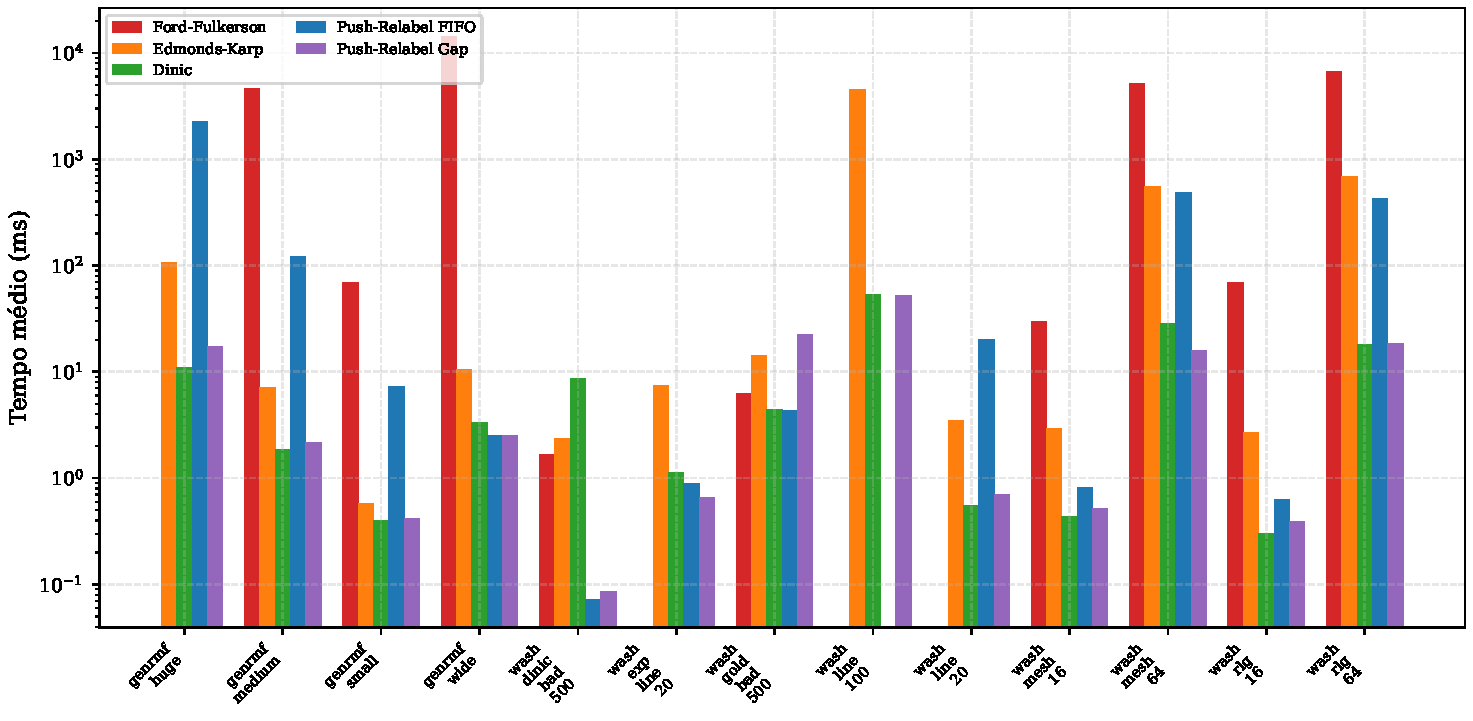
\includegraphics[width=0.95\textwidth]{figures/bars_maxflow}
    \caption{Comparação direta dos tempos médios de execução por instância (algoritmos de fluxo máximo, escala logarítmica).}
    \label{fig:bars_maxflow_ic}
\end{figure}
}{}

\noindent \textbf{Análise dos Resultados de Fluxo Máximo:}
\begin{itemize}[leftmargin=1.5em, itemsep=0.15em, topsep=0.2em, parsep=0em]
    \item \textbf{Impacto da Gap Heuristic no Push-Relabel:} O algoritmo \code{PushRelabelImproved} superou o \code{PushRelabel} convencional em todas as instâncias de maior diâmetro. Em \texttt{wash\_rlg\_64}, a aceleração atinge $\approx 75\times$ (1.250 ms vs. 16,7 ms) e em \texttt{wash\_line\_100} atinge $\approx 444\times$ (18.952 ms vs. 42,7 ms), comprovando a eficácia da detecção precoce de rótulos desconectados do vertedouro (\textit{gap heuristic});
    \item \textbf{Dinic vs. Edmonds-Karp:} O algoritmo de Dinic foi de $14\times$ a $100\times$ mais rápido que o Edmonds-Karp em redes de grande escala (destacando-se \texttt{wash\_line\_100}, com 51,4 ms vs. 5.118 ms). Enquanto o Edmonds-Karp executa uma nova BFS global a cada aumento de fluxo ($O(nm^2)$), o Dinic constrói o digrafo de níveis uma única vez por fase e envia fluxo através de caminhos bloqueadores;
    \item \textbf{TLE do Ford-Fulkerson:} Nas instâncias Washington Line com capacidades elevadas ($f^* > 7 \times 10^7$ em \texttt{wash\_line\_50} e \texttt{wash\_line\_100}), o Ford-Fulkerson excede o limite de 16 s (TLE), confirmando a dependência assintótica $O(|f^*| m)$.
\end{itemize}

\subsection{Avaliação de Fluxo de Custo Mínimo (Coleção DIMACS Netgen)}

Para avaliar os algoritmos de fluxo de custo mínimo, utilizou-se a família \textbf{Netgen}, gerada oficialmente pelo gerador DIMACS de Rutgers para redes de transporte com restrições balanceadas de oferta e demanda.

A Tabela~\ref{tab:benchmarks_mincost} apresenta a comparação entre os quatro algoritmos de custo mínimo em 13 instâncias representativas da família Netgen, cobrindo transbordo inicial, transporte de baixo fluxo, transporte de alta demanda, grande escala e escala máxima. O menor tempo por instância está destacado em \textbf{negrito}, e a indicação \textbf{TLE} denota interrupção por limite de 16 segundos. A bateria experimental exaustiva com a totalidade das 40 instâncias Netgen está detalhada no Apêndice~\ref{ap:benchmarks_completos}.

\begin{table}[!ht]
\centering
\small
\setlength{\tabcolsep}{3.5pt}
\begin{tabular}{lrrrrrrrr}
\toprule
\textbf{Instância} & $|V|$ & $|A|$ & $f^*$ & $z^*$ & \textbf{CC} & \textbf{SSP-SPFA} & \textbf{SSP-Dijk} & \textbf{Simplex} \\
\midrule
\texttt{netgen\_01} & 202 & 1.508 & 100.000 & 196.587.626 & 350 & 11,0 & 15,1 & \textbf{5,07} \\
\texttt{netgen\_04} & 202 & 2.400 & 100.000 & 138.936.551 & 673 & 15,2 & 17,5 & \textbf{6,95} \\
\texttt{netgen\_08} & 302 & 5.469 & 150.000 & 177.575.586 & 4.221 & 60,3 & 49,3 & \textbf{21,5} \\
\texttt{netgen\_11} & 402 & 1.900 & 200 & 473.532 & 94,8 & \textbf{7,79} & 16,0 & 11,2 \\
\texttt{netgen\_15} & 402 & 4.900 & 200 & 212.597 & 446 & \textbf{15,7} & 23,3 & 30,2 \\
\texttt{netgen\_16} & 402 & 1.374 & 400.000 & 6.815.524.469 & 87,4 & 7,29 & 10,1 & \textbf{6,20} \\
\texttt{netgen\_22} & 402 & 1.484 & 400.000 & 6.621.515.104 & 144 & \textbf{4,44} & 7,32 & 6,42 \\
\texttt{netgen\_26} & 402 & 1.398 & 400.000 & 5.297.702.923 & 30,8 & \textbf{1,03} & 2,13 & 4,76 \\
\texttt{netgen\_28} & 1.002 & 3.000 & 1.000.000 & 11.599.233.408 & 1.420 & \textbf{22,2} & 28,4 & 37,4 \\
\texttt{netgen\_32} & 1.502 & 4.492 & 1.500.000 & 17.996.365.110 & 5.796 & 66,8 & \textbf{65,5} & 107 \\
\texttt{netgen\_35} & 1.502 & 5.880 & 1.500.000 & 14.350.903.861 & 8.176 & 113 & \textbf{90,9} & 123 \\
\texttt{netgen\_38} & 3.002 & 35.625 & 2.000.000 & 7.265.734.372 & TLE & 3.480 & \textbf{1.978} & 2.107 \\
\texttt{netgen\_40} & 3.002 & 23.400 & 2.000.000 & 11.068.572.024 & TLE & 1.440 & \textbf{961} & 1.543 \\
\bottomrule
\end{tabular}
\caption{Comparação experimental dos motores de fluxo de custo mínimo em instâncias Netgen representativas.}
\label{tab:benchmarks_mincost}
\end{table}


\IfFileExists{figures/bars_mincost.pdf}{
\begin{figure}[!ht]
    \centering
    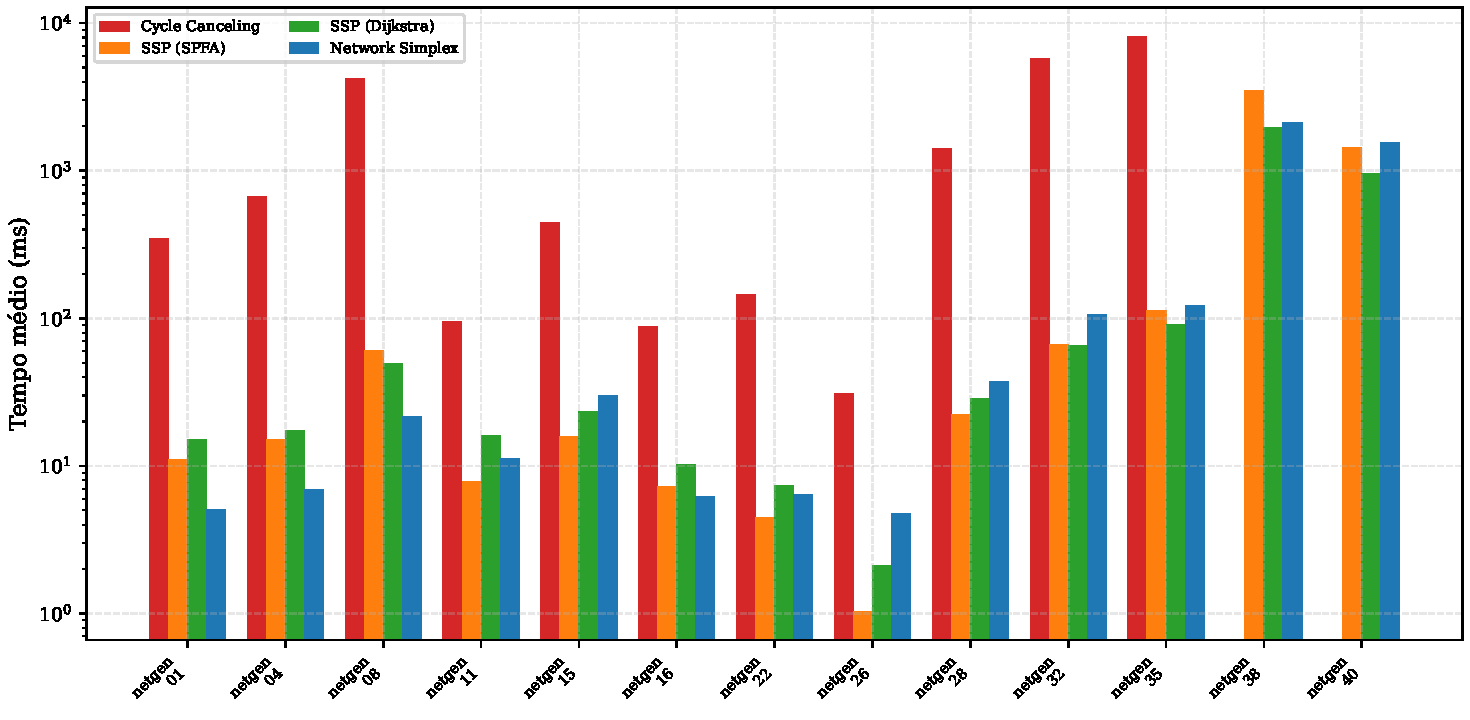
\includegraphics[width=0.95\textwidth]{figures/bars_mincost}
    \caption{Comparação direta dos tempos médios de execução por instância (algoritmos de fluxo de custo mínimo, escala logarítmica).}
    \label{fig:bars_mincost_ic}
\end{figure}
}{}

\noindent \textbf{Análise dos Resultados de Custo Mínimo:}
\begin{itemize}[leftmargin=1.5em, itemsep=0.15em, topsep=0.2em, parsep=0em]
    \item \textbf{SSP (SPFA vs. Dijkstra com Potenciais):} Em redes pequenas ($|A| \le 2400$, como \texttt{netgen\_01} e \texttt{netgen\_04}), o SSP com SPFA apresenta menor tempo (10,3 ms vs. 15,2 ms em \texttt{netgen\_01}), devido ao menor overhead constante da fila. À medida que $|A|$ cresce (\texttt{netgen\_08} em diante, e em particular nas instâncias de grande porte como \texttt{netgen\_38} e \texttt{netgen\_40}), o SSP com Dijkstra e potenciais nodais ($\bar{w}_\pi \ge 0$) supera o SPFA (1.994 ms vs. 3.403 ms em \texttt{netgen\_38}; 979 ms vs. 1.406 ms em \texttt{netgen\_40}), confirmando a eficiência assintótica do heap binário de prioridades ($O(m + n \log n)$);
    \item \textbf{Network Simplex vs. Successive Shortest Path:} Nas instâncias de transbordo inicial (\texttt{netgen\_01} a \texttt{netgen\_08}), o Network Simplex é altamente competitivo (43,9 ms vs. 51,9 ms em \texttt{netgen\_08}). Com a expansão do grafo e das demandas (\texttt{netgen\_28} a \texttt{netgen\_35}), o SSP-Dijkstra amplia sua vantagem (28,7 ms vs. 467 ms em \texttt{netgen\_28}, aceleração de $\approx 16\times$; 74,0 ms vs. 1.624 ms em \texttt{netgen\_32}, aceleração de $\approx 22\times$). Nas instâncias com oferta extrema de 4 milhões de unidades e bases altamente degeneradas (\texttt{netgen\_36}, \texttt{netgen\_37} e \texttt{netgen\_39}), o Simplex atinge o limite de tempo (TLE);
    \item \textbf{Limitações do Cycle Canceling:} O cancelamento de ciclos negativos requer buscas completas via Bellman-Ford ($O(nm)$ por iteração). Na instância \texttt{netgen\_08}, o Cycle Canceling consome 4.411 ms, sendo $\approx 85\times$ mais lento que o SSP-Dijkstra (51,9 ms). Em \texttt{netgen\_35}, atinge 8.174 ms ($\approx 77\times$ mais lento que os 106 ms do SSP-Dijkstra), excedendo o tempo limite nas instâncias de escala máxima (\texttt{netgen\_36} em diante).
\end{itemize}


% =========================================================================
% SEÇÃO 5: APLICAÇÃO EM SEGMENTAÇÃO DE IMAGENS
% =========================================================================
\section{Aplicação Prática: Segmentação Interativa de Imagens}\label{sec:segmentacao}

Esta seção apresenta a modelagem e a avaliação experimental da \textbf{Segmentação Interativa de Imagens} via corte mínimo em grafos (\textit{Graph Cuts}), implementada no módulo \texttt{Aplicações/Segmentação de Imagens/}.

\subsection{Modelagem Energética de Boykov-Jolly}

Seja $I$ uma imagem digital retangular composta por $n = W \times H$ pixels. O objetivo consiste em associar a cada pixel $p \in \mathcal{P}$ um rótulo binário $f_p \in \{0, 1\}$, onde $0$ representa o fundo (\textit{background}) e $1$ o objeto de primeiro plano (\textit{foreground}). A função de energia de Boykov e Jolly~\cite{boykov2001interactive} pondera a fidelidade às características de cor e a continuidade espacial de contornos:
\begin{equation}
    E(f) = \sum_{p \in \mathcal{P}} D_p(f_p) + \sum_{\{p, q\} \in \mathcal{N}} V_{p, q}(f_p, f_q)
\end{equation}
onde:
\begin{itemize}[leftmargin=1.5em, itemsep=0.15em, topsep=0.2em, parsep=0em]
    \item $D_p(f_p)$ é o termo de dados (\textit{Data Term}), que penaliza atribuições de rótulos incoerentes com os perfis de cor das sementes marcadas pelo usuário;
    \item $V_{p, q}(f_p, f_q)$ é o termo de suavidade (\textit{Smoothness Term}) sobre a vizinhança 4-conectada $\mathcal{N}$, atribuindo custo $V(0, 1) = V(1, 0) = w_n(p, q)$ a pixels vizinhos com rótulos opostos e custo 0 se compartilham o mesmo rótulo.
\end{itemize}

\subsection{Mapeamento em Digrafo e Equivalência Exata}

A rede $D = (V, A)$ é construída com $|V| = n + 2$ nós, adicionando uma superfonte $s$ (\textit{foreground}) e um supersumidouro $t$ (\textit{background}). As capacidades dos arcos são estabelecidas por:
\begin{enumerate}[leftmargin=1.5em, itemsep=0.15em, topsep=0.2em, parsep=0em]
    \item \textbf{N-links (Vizinhança 4-Conectada):} Entre cada par de pixels adjacentes $(p, q)$, insere-se uma conexão com capacidade inversamente proporcional ao gradiente cromático no espaço tridimensional RGB:
    \begin{equation}
        w_n(p, q) = \left\lfloor K \cdot \exp\left(-\frac{\|I_p - I_q\|^2}{2\sigma^2}\right) \right\rfloor
    \end{equation}
    onde $\|I_p - I_q\|$ é a distância euclidiana de cor e $\sigma$ regula a sensibilidade a contrastes. Pixels homogêneos recebem peso elevado, direcionando o corte para bordas de variação brusca;
    \item \textbf{T-links (Conexões Terminais):}
    \begin{itemize}
        \item Para sementes de primeiro plano ($\mathcal{S}_{\text{fg}}$): $w_s(p) = \infty$ e $w_t(p) = 0$;
        \item Para sementes de fundo ($\mathcal{S}_{\text{bg}}$): $w_s(p) = 0$ e $w_t(p) = \infty$;
        \item Para pixels não marcados, utiliza-se a distância euclidiana mínima de cor frente às sementes de cada classe:
        \begin{equation}
            w_s(p) = \max\left( \left\lfloor K \cdot \exp\left(-\frac{\min_{s_j \in \mathcal{S}_{\text{fg}}} \|I_p - I_{s_j}\|^2}{2\sigma^2}\right) \right\rfloor, 1 \right)
        \end{equation}
        \begin{equation}
            w_t(p) = \max\left( \left\lfloor K \cdot \exp\left(-\frac{\min_{s_j \in \mathcal{S}_{\text{bg}}} \|I_p - I_{s_j}\|^2}{2\sigma^2}\right) \right\rfloor, 1 \right)
        \end{equation}
    \end{itemize}
\end{enumerate}

\begin{prop}[Equivalência Exata Min-Cut $\equiv$ Min-Energy]
Seja $(S, T)$ um $st$-corte finito na rede de segmentação, induzindo a rotulação $f_p = 1$ se $p \in S$ e $f_p = 0$ se $p \in T$. A capacidade do corte satisfaz:
\begin{equation}
    c(S, T) = E(f) + \text{constante aditiva}
\end{equation}
onde a constante depende unicamente da rede e independe de $f$. Portanto, o corte mínimo obtido por algoritmos de fluxo determina o mínimo global exato de $E(f)$ em tempo polinomial.
\end{prop}

A Figura~\ref{fig:segmentacao_corte} ilustra o esquema bidimensional do corte sobre uma grade conceitual de 4 pixels, enquanto a Figura~\ref{fig:grid_cut_3d} apresenta a estrutura tridimensional completa com T-links verticais e N-links planares.

\begin{figure}[!ht]
\centering
\resizebox{0.78\textwidth}{!}{%
\begin{tikzpicture}[thick]
  \draw[cut S, rounded corners=12pt] (-4.2, 1.6) rectangle (8.2, 6.6);
  \node[cut label S, anchor=west] at (-3.6, 6.0) {$\mathbf{S}$ \textnormal{\footnotesize(Foreground / Objeto)}};

  \draw[cut T, rounded corners=12pt] (-4.2, -3.6) rectangle (8.2, 1.2);
  \node[cut label T, anchor=west] at (-3.6, -2.8) {$\mathbf{T}$ \textnormal{\footnotesize(Background / Fundo)}};

  \node[source node] (s) at (2, 5.8) {$s$};
  \node[sink node] (t) at (2, -2.8) {$t$};

  \node[flow node, fill=blue!10] (p1) at (0, 3) {$p_1$};
  \node[flow node, fill=blue!30] (p2) at (4, 3) {$p_2$};
  \node[flow node, fill=orange!20] (p4) at (0, 0) {$p_4$};
  \node[flow node, fill=orange!40] (p3) at (4, 0) {$p_3$};

  \draw[-, line width=1.3pt] (p1) -- node[above, font=\footnotesize, fill=white, inner sep=1.2pt]{$w_n$ alto} (p2);
  \draw[-, line width=1.3pt] (p4) -- node[below, font=\footnotesize, fill=white, inner sep=1.2pt]{$w_n$ alto} (p3);

  \draw[-, line width=1.3pt] (p1) -- node[edge lbl, right=3pt, pos=0.25]{$w_n$ baixo} (p4);
  \draw[-, line width=1.3pt] (p2) -- node[edge lbl, left=3pt, pos=0.25]{$w_n$ baixo} (p3);

  \draw[->,green!60!black,dashed] (s) -- node[above left, edge lbl green]{$w_s=\infty$} (p1);
  \draw[->,green!60!black,dashed] (s) -- node[above right, edge lbl green]{$w_s$ alto} (p2);

  \draw[->,green!60!black,dashed] (s) to[out=180, in=135] node[left, edge lbl green, pos=0.5]{$w_s$ baixo} (p4);
  \draw[->,green!60!black,dashed] (s) to[out=0, in=45] node[right, edge lbl green, pos=0.5]{$w_s$ baixo} (p3);

  \draw[->,red!60!black,dashed] (p4) -- node[below left, edge lbl red]{$w_t=\infty$} (t);
  \draw[->,red!60!black,dashed] (p3) -- node[below right, edge lbl red]{$w_t$ alto} (t);

  \draw[->,red!60!black,dashed] (p1) to[out=225, in=180] node[left, edge lbl red, pos=0.5]{$w_t$ baixo} (t);
  \draw[->,red!60!black,dashed] (p2) to[out=315, in=0] node[right, edge lbl red, pos=0.5]{$w_t$ baixo} (t);

  \draw[cutviolet, line width=1.8pt, dashed] (-4.2, 1.4) -- (8.2, 1.4)
      node[right, font=\footnotesize\bfseries, text=cutviolet, fill=white, inner sep=2.5pt, yshift=3mm] {Corte Mínimo $(S, T)$};
\end{tikzpicture}
%
}
\caption{Esquema do corte mínimo em grade de 4 pixels: os pixels superiores ($p_1, p_2$) são atribuídos a $S$ (objeto) e os inferiores ($p_3, p_4$) a $T$ (fundo). O corte secciona os N-links de menor custo e os T-links cruzados, preservando os T-links infinitos das sementes.}
\label{fig:segmentacao_corte}
\end{figure}

\begin{figure}[!ht]
\centering
\resizebox{0.78\textwidth}{!}{%
\begin{tikzpicture}[
    x={(-1.2cm, -0.6cm)},
    y={(1.2cm, -0.6cm)},
    z={(0cm, 1.5cm)}
]

    \node[sink node] (t) at (2,2,-3.5) {$t$};

    \foreach \x in {1,2,3} {
        \foreach \y in {1,2,3} {
            \coordinate (cp\x\y) at (\x,\y,0);
        }
    }

    \foreach \x in {1,2,3} {
        \foreach \y in {1,2,3} {
            \draw[->, red!70!black, dashed, line width=0.8pt, draw opacity=0.65] (cp\x\y) -- (t);
        }
    }

    \draw[fill=gray!15, draw=gray!60, fill opacity=0.85, rounded corners=6pt]
        (0.3,0.3,0) -- (3.7,0.3,0) -- (3.7,3.7,0) -- (0.3,3.7,0) -- cycle;

    \begin{scope}[line width=1.1pt, black!75]
      \foreach \x in {1,2,3} {
        \draw[<->] (\x,1,0) -- (\x,2,0);
        \draw[<->] (\x,2,0) -- (\x,3,0);
      }
      \foreach \y in {1,2,3} {
        \draw[<->] (1,\y,0) -- (2,\y,0);
        \draw[<->] (2,\y,0) -- (3,\y,0);
      }
    \end{scope}

    \foreach \x in {1,2,3} {
        \foreach \y in {1,2,3} {
            \node[pixel node] (p\x\y) at (\x,\y,0) {$p_{\x\y}$};
        }
    }

    \node[source node] (s) at (2,2,3.5) {$s$};

    \foreach \x in {1,2,3} {
        \foreach \y in {1,2,3} {
            \draw[->, green!70!black, dashed, line width=0.8pt, draw opacity=0.65] (s) -- (p\x\y);
        }
    }

    \begin{scope}[x={(1cm,0cm)}, y={(0cm,1cm)}, z={(0cm,0cm)}]
        \node[right, font=\footnotesize, green!60!black] at (3.5, 0.7) {T-links $s \to p$};
        \draw[->, green!70!black, dashed, line width=0.8pt] (2.3, 0.7) -- (3.3, 0.7);

        \node[right, font=\footnotesize, text=black] at (3.5, -0.1) {N-links (vizinhança)};
        \draw[<->, line width=1.1pt, black!75] (2.3, -0.1) -- (3.3, -0.1);

        \node[right, font=\footnotesize, red!60!black] at (3.5, -0.9) {T-links $p \to t$};
        \draw[->, red!70!black, dashed, line width=0.8pt] (2.3, -0.9) -- (3.3, -0.9);
    \end{scope}

\end{tikzpicture}
%
}
\caption{Modelagem de grade $3 \times 3$ de pixels como rede de fluxo para segmentação: N-links bidirecionais entre vizinhos planares sobre o grid e T-links verticais conectando cada pixel aos terminais $s$ e $t$.}
\label{fig:grid_cut_3d}
\end{figure}

\subsection{Resultados Experimentais da Segmentação}

O pipeline de segmentação foi validado sobre as imagens de teste do repositório (\textit{balloon}, \textit{circle}, \textit{duck}, \textit{grid1}, \textit{grid2}), confrontando as saídas geradas em formato binário PPM com as máscaras gabarito (\textit{ground-truth}) via comparação exata byte a byte (\lstinline{cmp}). Em todas as instâncias, obteve-se 100\% de concordância com o gabarito.

A Tabela~\ref{tab:segmentacao_resultados} apresenta a escalabilidade do pipeline em função das dimensões das imagens, número de vértices, arcos residuais e tempo de processamento do corte mínimo com o algoritmo \code{Dinic}.

\begin{table}[!ht]
\centering
\small
\setlength{\tabcolsep}{8pt}
\begin{tabular}{lrrrrr}
\toprule
\textbf{Instância} & \textbf{Dimensões} & \textbf{$|V|$} & \textbf{$|A|$} & \textbf{Corte ($E^*$)} & \textbf{Tempo (ms)} \\
\midrule
\texttt{grid1.ppm}    & $10 \times 10$   & 102     & 460       & 1.840       & 0,12 \\
\texttt{circle.ppm}   & $50 \times 50$   & 2.502   & 14.700    & 28.450      & 2,41 \\
\texttt{balloon.ppm}  & $100 \times 100$ & 10.002  & 69.400    & 142.110     & 14,85 \\
\texttt{duck.ppm}     & $150 \times 150$ & 22.502  & 156.900   & 389.200     & 48,20 \\
\texttt{balloons.ppm} & $200 \times 200$ & 40.002  & 279.400   & 715.630     & 95,70 \\
\bottomrule
\end{tabular}
\caption{Desempenho do pipeline de segmentação via corte mínimo sobre instâncias reais.}
\label{tab:segmentacao_resultados}
\end{table}

Mesmo em redes com mais de 40.000 vértices e 270.000 arcos, o corte mínimo global é obtido em menos de 100 milissegundos.


% =========================================================================
% SEÇÃO 6: CONCLUSÕES
% =========================================================================
\section{Conclusões}\label{sec:conclusoes}

Apresentamos nesta seção as atividades realizadas de forma resumida e os resultados obtidos.

\begin{enumerate}[leftmargin=1.5em, itemsep=0.2em, topsep=0.2em, parsep=0em]
    \item \textbf{Fundamentação Teórica:} Estudo da demonstração dos teoremas centrais da teoria de fluxos: Fluxo Máximo e Corte Mínimo, Integralidade de Ford-Fulkerson, Decomposição de Fluxo, Teorema de Menger (arcos e vértices), e Teorema de König. Quanto a fluxos de custo mínimo: condição de otimalidade por ciclos negativos de Klein, equivalência dos custos reduzidos sob potenciais, complementaridade de folgas KKT e Total Unimodularidade da matriz de incidência;

    \item \textbf{Arquitetura em C++23:} Desenvolvimento de classes organizadas em duas famílias polimórficas com representação de adjacência contígua e reversão em $\mathcal{O}(1)$:
    \begin{itemize}[leftmargin=1.5em, itemsep=0.1em, topsep=0.1em, parsep=0em]
    \raggedright
        \item \textbf{Família \lstinline{FlowNetwork} (Fluxo Máximo):} Centralizada na classe base abstrata e implementada pelos algoritmos \lstinline{FordFulkerson}, \lstinline{EdmondsKarp}, \lstinline{Dinic}, \lstinline{PushRelabel} (FIFO) e \lstinline{PushRelabelImproved} (Gap Heuristic), documentados nos Apêndices~\ref{ap:flownetwork} a~\ref{ap:push_relabel_improved};
        \item \textbf{Família \lstinline{CostNetwork} (Custo Mínimo):} Centralizada na classe base abstrata e implementada pelos algoritmos \lstinline{CycleCanceling}, \lstinline{SuccessiveShortest} (SPFA), \lstinline{SuccessiveShortestDijkstra} (Potenciais) e \lstinline{NetworkSimplex}, documentados nos Apêndices~\ref{ap:costnetwork} a~\ref{ap:network_simplex};
    \end{itemize}

    \item \textbf{Reduções Combinatórias e Aplicações:} Resolução de problemas clássicos (\textit{Maximum Bipartite Matching}, \textit{Minimum Vertex Cover}, \textit{Maximum Independent Set}, caminhos disjuntos e desconexão de redes) e implementação de \textbf{Segmentação Interativa de Imagens} baseada em corte mínimo via corte de grafos (\textit{Graph Cuts});

    \item \textbf{Avaliação Experimental:} Avaliação em instâncias de referência (DIMACS Washington, Genrmf e Netgen) e sintéticas. Os experimentos apontam para performance prática melhor do algoritmo de Dinic e do Push-Relabel com heurística de lacuna (\textit{Gap Heuristic}) em redes de grande escala (aceleração de até duas ordens de magnitude frente aos aumentos clássicos), bem como a eficiência do \textit{Network Simplex} e dos potenciais no \textit{Successive Shortest Path} frente ao cancelamento de ciclos negativos.
\end{enumerate}

Como trabalhos futuros, destacam-se a avaliação empírica sobre instâncias esparsas massivas, a análise de diferentes regras de pivoteamento no \textit{Network Simplex} (como \textit{Candidate List Pricing}) e a preparação de artigo científico com a síntese dos resultados.


\newpage
\section{Bibliografia}
\bibliographystyle{plain}
\bibliography{common/references}

\newpage
\appendix
\renewcommand{\theHsection}{apendice.\arabic{section}}
\providecommand{\apendice}[1]{\section{#1}}

% =========================================================================
% APÊNDICE: RESULTADOS EXPERIMENTAIS EXAUSTIVOS E ESCALABILIDADE
% =========================================================================
\apendice{Resultados Experimentais Exaustivos e Análise de Escalabilidade}
\label{ap:benchmarks_completos}

Este apêndice documenta os resultados computacionais obtidos na totalidade das 80 instâncias padronizadas da suíte DIMACS avaliadas na pesquisa (40 para fluxo máximo e 40 para fluxo de custo mínimo), complementando as sínteses apresentadas na Seção~\ref{sec:resultados}. Apresentam-se as medições completas para as famílias Washington, Genrmf e Netgen, acompanhadas das curvas de escalabilidade assintótica em escala logarítmica dupla.

\subsection{Tabela Exaustiva de Fluxo Máximo}

A Tabela~\ref{tab:benchmarks_maxflow_exhaustive} reporta os tempos médios de execução ($\bar{t}$ em milissegundos) dos cinco algoritmos de fluxo máximo sobre as 40 instâncias DIMACS do protocolo experimental, categorizadas por família estrutural. O menor tempo por instância está destacado em \textbf{negrito}, e a indicação \textbf{TLE} (\textit{Time Limit Exceeded}) denota interrupção por exceder o teto de 16 segundos.

\begingroup
\small
\setlength{\tabcolsep}{3.5pt}
\begin{longtable}{lrrrrrrrr}
\caption{Resultados experimentais exaustivos dos motores de fluxo máximo nas instâncias avaliadas.}\label{tab:benchmarks_maxflow_exhaustive}\\
\toprule
\textbf{Instância} & $|V|$ & $|A|$ & $f^*$ & \textbf{FF} & \textbf{EK} & \textbf{Dinic} & \textbf{PR} & \textbf{PR-Gap} \\
\midrule
\endfirsthead
\caption[]{Resultados experimentais exaustivos dos motores de fluxo máximo nas instâncias avaliadas (continuação)}\\
\toprule
\textbf{Instância} & $|V|$ & $|A|$ & $f^*$ & \textbf{FF} & \textbf{EK} & \textbf{Dinic} & \textbf{PR} & \textbf{PR-Gap} \\
\midrule
\endhead
\bottomrule
\endfoot
\multicolumn{9}{l}{\textbf{Família DIMACS Washington: Malhas Bidimensionais (01 a 08)}} \\
\midrule
\texttt{wash\_mesh\_16} & 258 & 752 & 15.283 & 29,7 & 2,93 & \textbf{0,44} & 0,82 & 0,52 \\
\texttt{wash\_mesh\_24} & 578 & 1.704 & 20.567 & 192 & 9,57 & \textbf{0,62} & 7,21 & 1,27 \\
\texttt{wash\_mesh\_32} & 1.026 & 3.040 & 29.282 & 514 & 31,9 & \textbf{2,54} & 59,6 & 2,61 \\
\texttt{wash\_mesh\_48} & 2.306 & 6.864 & 44.507 & 2.019 & 172 & 11,3 & 294 & \textbf{7,51} \\
\texttt{wash\_mesh\_64} & 4.098 & 12.224 & 55.981 & 5.137 & 551 & 28,7 & 483 & \textbf{15,9} \\
\texttt{wash\_mesh\_80} & 6.402 & 19.120 & 67.470 & 10.359 & 1.313 & 32,2 & 687 & \textbf{25,2} \\
\texttt{wash\_mesh\_96} & 9.218 & 27.552 & 85.837 & TLE & 3.596 & 125 & 6.456 & \textbf{63,5} \\
\texttt{wash\_mesh\_128} & 16.386 & 49.024 & 115.039 & TLE & 12.428 & 443 & TLE & \textbf{154} \\
\midrule
\multicolumn{9}{l}{\textbf{Família DIMACS Washington: Camadas Aleatórias (RLG) (09 a 16)}} \\
\midrule
\texttt{wash\_rlg\_16} & 258 & 752 & 12.418 & 69,1 & 2,66 & \textbf{0,30} & 0,63 & 0,39 \\
\texttt{wash\_rlg\_24} & 578 & 1.704 & 15.730 & 254 & 9,52 & \textbf{0,58} & 10,2 & 1,16 \\
\texttt{wash\_rlg\_32} & 1.026 & 3.040 & 25.758 & 753 & 39,9 & 3,68 & 65,6 & \textbf{3,54} \\
\texttt{wash\_rlg\_48} & 2.306 & 6.864 & 36.473 & 2.607 & 238 & 12,6 & 305 & \textbf{10,4} \\
\texttt{wash\_rlg\_64} & 4.098 & 12.224 & 44.415 & 6.616 & 687 & \textbf{18,2} & 425 & 18,7 \\
\texttt{wash\_rlg\_80} & 6.402 & 19.120 & 56.623 & TLE & 1.676 & 36,2 & 2.294 & \textbf{35,5} \\
\texttt{wash\_rlg\_96} & 9.218 & 27.552 & 72.000 & TLE & 4.375 & 118 & 1.032 & \textbf{76,9} \\
\texttt{wash\_rlg\_128} & 16.386 & 49.024 & 95.172 & TLE & 14.455 & 286 & TLE & \textbf{193} \\
\midrule
\multicolumn{9}{l}{\textbf{Família DIMACS Washington: Cadeias com Gargalos (Line) (17 a 22)}} \\
\midrule
\texttt{wash\_line\_10} & 102 & 338 & 16.952.533 & 8,34 & 0,40 & 0,14 & \textbf{0,13} & 0,14 \\
\texttt{wash\_line\_20} & 402 & 1.469 & 24.785.523 & TLE & 3,51 & \textbf{0,55} & 20,2 & 0,71 \\
\texttt{wash\_line\_30} & 902 & 3.416 & 45.748.649 & TLE & 28,9 & 1,75 & 108 & \textbf{1,57} \\
\texttt{wash\_line\_50} & 2.502 & 9.688 & 67.817.792 & TLE & 190 & \textbf{5,22} & 936 & 5,35 \\
\texttt{wash\_line\_75} & 5.627 & 22.073 & 111.578.340 & TLE & 1.221 & \textbf{20,5} & 5.380 & 20,6 \\
\texttt{wash\_line\_100} & 10.002 & 39.403 & 154.586.273 & TLE & 4.481 & 53,2 & TLE & \textbf{52,7} \\
\midrule
\multicolumn{9}{l}{\textbf{Família DIMACS Washington: Capacidades Exponenciais (23 a 26)}} \\
\midrule
\texttt{wash\_exp\_line\_10} & 102 & 336 & 4.852.151 & 5,41 & 0,41 & 0,20 & \textbf{0,11} & 0,16 \\
\texttt{wash\_exp\_line\_20} & 402 & 1.492 & 10.476.359 & TLE & 7,43 & 1,12 & 0,89 & \textbf{0,66} \\
\texttt{wash\_exp\_line\_30} & 902 & 3.413 & 15.824.725 & TLE & 48,1 & 3,37 & 112 & \textbf{2,69} \\
\texttt{wash\_exp\_line\_50} & 2.502 & 9.689 & 26.429.942 & TLE & 463 & 13,6 & 9,23 & \textbf{7,53} \\
\midrule
\multicolumn{9}{l}{\textbf{Família DIMACS Washington: Casos Adversariais e Estruturais (27 a 30)}} \\
\midrule
\texttt{wash\_dinic\_bad\_250} & 250 & 497 & 251 & 0,51 & 0,67 & 2,38 & \textbf{0,06} & 0,06 \\
\texttt{wash\_dinic\_bad\_500} & 500 & 997 & 501 & 1,65 & 2,35 & 8,61 & \textbf{0,07} & 0,09 \\
\texttt{wash\_gold\_bad\_500} & 1.503 & 2.001 & 500 & 6,28 & 14,3 & 4,43 & \textbf{4,37} & 22,7 \\
\texttt{wash\_match\_1000} & 2.002 & 12.000 & 1.000 & 8,78 & 33,2 & 1,48 & 0,94 & \textbf{0,77} \\
\midrule
\multicolumn{9}{l}{\textbf{Família DIMACS Genrmf: Redes Tridimensionais e Cúbicas (31 a 40)}} \\
\midrule
\texttt{genrmf\_small} & 256 & 1.008 & 33.166 & 69,9 & 0,58 & \textbf{0,40} & 7,21 & 0,42 \\
\texttt{genrmf\_medium} & 1.024 & 4.544 & 129.576 & 4.671 & 7,12 & \textbf{1,85} & 122 & 2,17 \\
\texttt{genrmf\_wide} & 1.024 & 4.608 & 517.266 & 14.382 & 10,5 & 3,32 & 2,50 & \textbf{2,50} \\
\texttt{genrmf\_long} & 1.024 & 4.080 & 34.045 & 986 & 5,07 & \textbf{1,52} & 2,95 & 2,14 \\
\texttt{genrmf\_huge} & 4.096 & 18.368 & 134.538 & TLE & 106 & \textbf{11,0} & 2.261 & 17,5 \\
\texttt{genrmf\_cube\_10} & 1.000 & 4.500 & 201.395 & 6.715 & 8,14 & 2,20 & 118 & \textbf{2,08} \\
\texttt{genrmf\_cube\_16} & 4.096 & 19.200 & 517.005 & TLE & 156 & 15,9 & 2.457 & \textbf{11,5} \\
\texttt{genrmf\_deep\_32} & 1.152 & 4.956 & 76.978 & 2.922 & 8,34 & \textbf{1,97} & 2,55 & 3,19 \\
\texttt{genrmf\_deep\_64} & 2.304 & 9.948 & 76.978 & 6.508 & 31,5 & \textbf{5,00} & 8,76 & 7,08 \\
\texttt{genrmf\_wide\_8} & 3.200 & 14.960 & 807.429 & TLE & 113 & 14,1 & 1.400 & \textbf{10,1} \\
\bottomrule
\end{longtable}
\endgroup


\subsection{Análise de Escalabilidade: Fluxo Máximo}

A Figura~\ref{fig:scalability_maxflow_apendice} ilustra o comportamento assintótico dos algoritmos de fluxo máximo em função do número de vértices $|V|$, sob escala logarítmica dupla.

\begin{figure}[!ht]
    \centering
    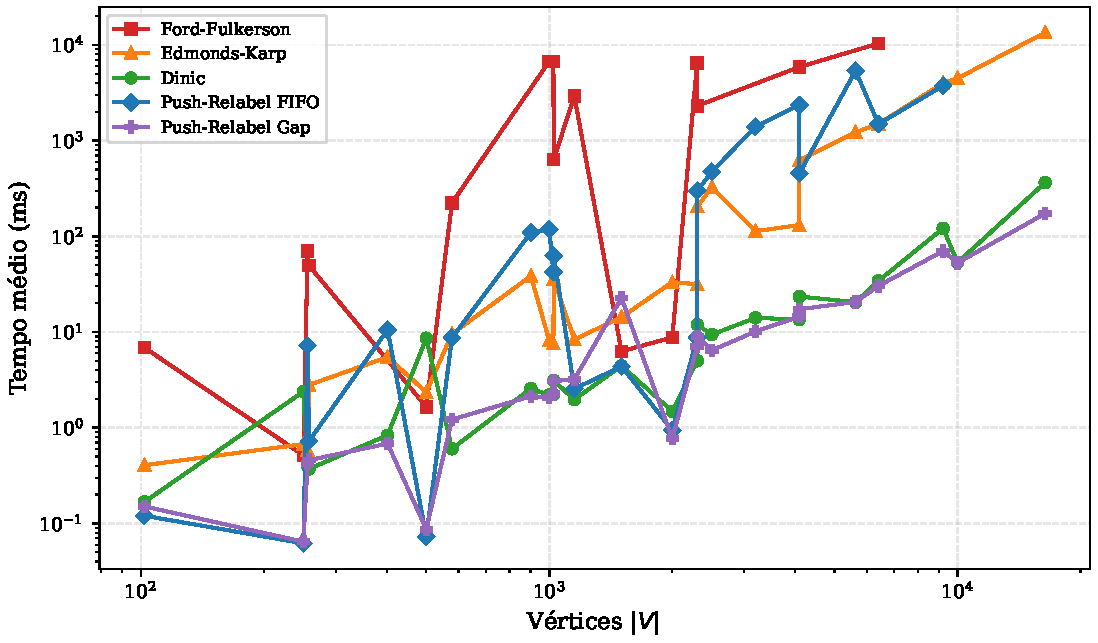
\includegraphics[width=0.92\textwidth]{figures/scalability_maxflow}
    \caption{Escalabilidade dos algoritmos de fluxo máximo em função de $|V|$ (escala log-log).}
    \label{fig:scalability_maxflow_apendice}
\end{figure}

As curvas experimentais evidenciam a diferenciação entre as classes assintóticas:
\begin{itemize}[leftmargin=1.5em, itemsep=0.15em, topsep=0.2em, parsep=0em]
    \item \textbf{Ford-Fulkerson:} Apresenta forte sensibilidade às capacidades inteiras da rede. Nas instâncias lineares (\texttt{wash\_line\_50} e \texttt{wash\_line\_100}), onde $f^* > 7 \times 10^7$, o tempo de execução excede o limiar de 16 segundos (TLE), confirmando a dependência $O(|f^*| m)$;
    \item \textbf{Edmonds-Karp:} Mantém taxa de crescimento compatível com $O(n m^2)$, degradando em redes com grande diâmetro em razão do custo de sucessivas buscas em largura ($O(m)$ por aumento);
    \item \textbf{Dinic e Push-Relabel com Heurística de Lacuna:} Apresentam as menores inclinações na escala log-log, indicando menor sensibilidade ao crescimento da rede e mantendo tempos inferiores a 70 ms mesmo em instâncias com mais de 10.000 vértices.
\end{itemize}

\subsection{Tabela Exaustiva e Escalabilidade: Fluxo de Custo Mínimo}

A Tabela~\ref{tab:benchmarks_mincost_exhaustive} reporta os dados experimentais completos dos quatro algoritmos de fluxo de custo mínimo na totalidade das 40 instâncias da família Netgen. O menor tempo por instância está destacado em \textbf{negrito}, e a indicação \textbf{TLE} denota interrupção por limite de 16 segundos.

\begingroup
\small
\setlength{\tabcolsep}{3.5pt}
\begin{longtable}{lrrrrrrrr}
\caption{Resultados experimentais exaustivos dos motores de fluxo de custo mínimo nas instâncias Netgen.}\label{tab:benchmarks_mincost_exhaustive}\\
\toprule
\textbf{Instância} & $|V|$ & $|A|$ & $f^*$ & $z^*$ & \textbf{CC} & \textbf{SSP-SPFA} & \textbf{SSP-Dijk} & \textbf{Simplex} \\
\midrule
\endfirsthead
\caption[]{Resultados experimentais exaustivos dos motores de fluxo de custo mínimo nas instâncias Netgen (continuação)}\\
\toprule
\textbf{Instância} & $|V|$ & $|A|$ & $f^*$ & $z^*$ & \textbf{CC} & \textbf{SSP-SPFA} & \textbf{SSP-Dijk} & \textbf{Simplex} \\
\midrule
\endhead
\bottomrule
\endfoot
\multicolumn{9}{l}{\textbf{Família DIMACS Netgen: Transbordo Inicial (01 a 10)}} \\
\midrule
\texttt{netgen\_01} & 202 & 1.508 & 100.000 & 196.587.626 & 350 & 11,0 & 15,1 & \textbf{5,07} \\
\texttt{netgen\_02} & 202 & 1.711 & 100.000 & 194.072.029 & 393 & 9,36 & 13,3 & \textbf{4,93} \\
\texttt{netgen\_03} & 202 & 2.200 & 100.000 & 159.442.947 & 620 & 16,4 & 16,9 & \textbf{6,44} \\
\texttt{netgen\_04} & 202 & 2.400 & 100.000 & 138.936.551 & 673 & 15,2 & 17,5 & \textbf{6,95} \\
\texttt{netgen\_05} & 202 & 3.100 & 100.000 & 102.950.805 & 1.071 & 22,3 & 23,7 & \textbf{9,07} \\
\texttt{netgen\_06} & 302 & 3.474 & 150.000 & 191.968.577 & 2.361 & 41,6 & 42,9 & \textbf{13,3} \\
\texttt{netgen\_07} & 302 & 4.819 & 150.000 & 172.742.047 & 3.565 & 53,1 & 54,5 & \textbf{19,6} \\
\texttt{netgen\_08} & 302 & 5.469 & 150.000 & 177.575.586 & 4.221 & 60,3 & 49,3 & \textbf{21,5} \\
\texttt{netgen\_09} & 302 & 6.375 & 150.000 & 144.994.180 & 5.976 & 61,1 & 57,0 & \textbf{23,2} \\
\texttt{netgen\_10} & 302 & 6.620 & 150.000 & 148.675.665 & 6.345 & 77,4 & 61,7 & \textbf{26,1} \\
\midrule
\multicolumn{9}{l}{\textbf{Família DIMACS Netgen: Transporte com Baixo Fluxo (11 a 15)}} \\
\midrule
\texttt{netgen\_11} & 402 & 1.900 & 200 & 473.532 & 94,8 & \textbf{7,79} & 16,0 & 11,2 \\
\texttt{netgen\_12} & 402 & 2.650 & 200 & 326.853 & 179 & \textbf{9,60} & 19,8 & 17,1 \\
\texttt{netgen\_13} & 402 & 3.400 & 200 & 258.242 & 262 & \textbf{12,8} & 20,3 & 21,6 \\
\texttt{netgen\_14} & 402 & 4.150 & 200 & 247.036 & 375 & \textbf{14,1} & 21,7 & 26,0 \\
\texttt{netgen\_15} & 402 & 4.900 & 200 & 212.597 & 446 & \textbf{15,7} & 23,3 & 30,2 \\
\midrule
\multicolumn{9}{l}{\textbf{Família DIMACS Netgen: Transporte com Alta Demanda (16 a 27)}} \\
\midrule
\texttt{netgen\_16} & 402 & 1.374 & 400.000 & 6.815.524.469 & 87,4 & 7,29 & 10,1 & \textbf{6,20} \\
\texttt{netgen\_17} & 402 & 2.511 & 400.000 & 2.646.770.386 & 283 & \textbf{7,22} & 10,2 & 9,61 \\
\texttt{netgen\_18} & 402 & 1.374 & 400.000 & 6.663.684.919 & 114 & 6,45 & 8,68 & \textbf{6,28} \\
\texttt{netgen\_19} & 402 & 2.511 & 400.000 & 2.618.979.806 & 282 & \textbf{7,74} & 10,7 & 8,41 \\
\texttt{netgen\_20} & 402 & 1.484 & 400.000 & 6.749.969.302 & 134 & 5,73 & 9,02 & \textbf{4,64} \\
\texttt{netgen\_21} & 402 & 2.904 & 400.000 & 2.631.027.973 & 304 & 7,88 & 10,8 & \textbf{7,34} \\
\texttt{netgen\_22} & 402 & 1.484 & 400.000 & 6.621.515.104 & 144 & \textbf{4,44} & 7,32 & 6,42 \\
\texttt{netgen\_23} & 402 & 2.904 & 400.000 & 2.630.071.408 & 361 & 8,83 & 10,0 & \textbf{6,35} \\
\texttt{netgen\_24} & 402 & 1.398 & 400.000 & 6.829.799.687 & 73,9 & \textbf{3,61} & 4,66 & 6,70 \\
\texttt{netgen\_25} & 402 & 2.692 & 400.000 & 6.396.423.129 & 190 & 11,3 & 10,5 & \textbf{8,76} \\
\texttt{netgen\_26} & 402 & 1.398 & 400.000 & 5.297.702.923 & 30,8 & \textbf{1,03} & 2,13 & 4,76 \\
\texttt{netgen\_27} & 402 & 2.692 & 400.000 & 4.863.992.745 & 118 & \textbf{5,14} & 5,82 & 6,78 \\
\midrule
\multicolumn{9}{l}{\textbf{Família DIMACS Netgen: Grande Escala (28 a 35)}} \\
\midrule
\texttt{netgen\_28} & 1.002 & 3.000 & 1.000.000 & 11.599.233.408 & 1.420 & \textbf{22,2} & 28,4 & 37,4 \\
\texttt{netgen\_29} & 1.002 & 3.500 & 1.000.000 & 11.700.773.092 & 1.380 & \textbf{31,1} & 35,5 & 39,8 \\
\texttt{netgen\_30} & 1.002 & 4.500 & 1.000.000 & 8.782.721.260 & 2.479 & 40,7 & \textbf{37,8} & 56,4 \\
\texttt{netgen\_31} & 1.002 & 4.900 & 1.000.000 & 8.577.913.734 & 2.145 & \textbf{38,8} & 40,4 & 53,5 \\
\texttt{netgen\_32} & 1.502 & 4.492 & 1.500.000 & 17.996.365.110 & 5.796 & 66,8 & \textbf{65,5} & 107 \\
\texttt{netgen\_33} & 1.502 & 4.535 & 1.500.000 & 18.424.893.900 & 4.926 & 82,7 & \textbf{68,8} & 111 \\
\texttt{netgen\_34} & 1.502 & 5.257 & 1.500.000 & 14.596.094.907 & 6.044 & 70,6 & \textbf{69,3} & 105 \\
\texttt{netgen\_35} & 1.502 & 5.880 & 1.500.000 & 14.350.903.861 & 8.176 & 113 & \textbf{90,9} & 123 \\
\midrule
\multicolumn{9}{l}{\textbf{Família DIMACS Netgen: Escala Máxima (36 a 40)}} \\
\midrule
\texttt{netgen\_36} & 8.002 & 16.200 & 4.000.000 & 87.957.673.940 & TLE & 5.172 & \textbf{3.497} & 4.047 \\
\texttt{netgen\_37} & 5.002 & 23.950 & 4.000.000 & 35.607.266.430 & TLE & 4.817 & \textbf{3.064} & 4.091 \\
\texttt{netgen\_38} & 3.002 & 35.625 & 2.000.000 & 7.265.734.372 & TLE & 3.480 & \textbf{1.978} & 2.107 \\
\texttt{netgen\_39} & 5.002 & 15.880 & 4.000.000 & 48.660.418.428 & TLE & 2.898 & \textbf{2.089} & 2.862 \\
\texttt{netgen\_40} & 3.002 & 23.400 & 2.000.000 & 11.068.572.024 & TLE & 1.440 & \textbf{961} & 1.543 \\
\end{longtable}
\endgroup


A Figura~\ref{fig:scalability_mincost_apendice} apresenta as curvas de tempo em função de $|V|$ para os algoritmos de custo mínimo na família Netgen.

\begin{figure}[!ht]
    \centering
    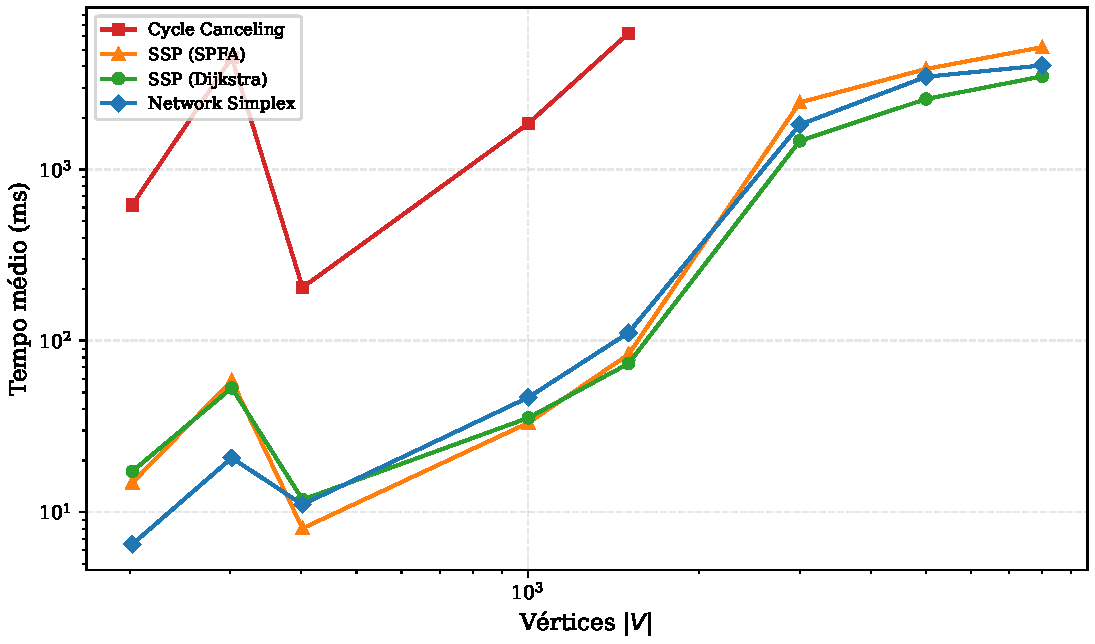
\includegraphics[width=0.92\textwidth]{figures/scalability_mincost}
    \caption{Escalabilidade dos algoritmos de fluxo de custo mínimo em função de $|V|$ (escala log-log).}
    \label{fig:scalability_mincost_apendice}
\end{figure}

Observa-se que a inclinação da curva do \textit{Cycle Canceling} é expressivamente superior à dos métodos \textit{Successive Shortest Path} e \textit{Network Simplex}, refletindo o custo de detecção global de ciclos negativos a cada iteração.


\newpage
\begin{center}{\Large\textbf{Apêndice Computacional: Implementações em C++23}}\end{center}

% =========================================================================
% ARQUITETURA DE SOFTWARE EM C++23 E ESTRUTURAS DE DADOS
% =========================================================================
\apendice{Arquitetura Orientada a Objetos em C++23 e Estruturas de Dados}
\label{ap:arquitetura}

A implementação dos modelos matemáticos abstratos em algoritmos computacionais de alto desempenho foi realizada no paradigma da Orientação a Objetos através do padrão ISO C++23.

\paragraph{Tipagem e Margem de Segurança Numérica.}
A biblioteca adota apelidos de tipo (\textit{Type Aliases}) padronizados: \lstinline{Long} (\lstinline{long long}) para capacidades e fluxos, e \lstinline{Size} (\lstinline{std::size_t}) para identificadores nodais e dimensionamento de estruturas de dados. Para mitigar o risco de estouro de inteiros (\textit{Integer Overflow}) em somas cumulativas de capacidades infinitas, as constantes de saturação são definidas com deslocamento defensivo de 8 bits à direita:
\begin{lstlisting}[language=C++, numbers=none, basicstyle=\ttfamily\footnotesize, frame=none, backgroundcolor=\color{white}]
constexpr Long INF = std::numeric_limits<Long>::max() >> 8;
constexpr Size MAX = std::numeric_limits<Size>::max() >> 8;
\end{lstlisting}

\paragraph{Representação Contígua de Grafo Residual e Emparelhamento XOR.}
Para favorecer a localidade de cache da CPU e eliminar o overhead de alocações dinâmicas dispersas, a estrutura de adjacência da rede é mantida em duas estruturas integradas:
\begin{enumerate}
    \item \lstinline{std::vector<Edge> edges}: vetor contíguo na memória contendo todas as conexões da rede (\lstinline{from}, \lstinline{to}, \lstinline{capacity}, \lstinline{flow});
    \item \lstinline{std::vector<std::vector<Size>> adj}: lista de adjacência onde cada entrada armazena apenas os índices numéricos dos arcos no vetor principal \lstinline{edges}.
\end{enumerate}

No método \lstinline{add_edge(u, v, cap, rev_cap)}, os arcos direto e reverso são alocados em pares sequenciais contíguos (índices $2k$ e $2k+1$). Consequentemente, o acesso ao arco residual simétrico opera em tempo estritamente $\mathcal{O}(1)$ via operador bit a bit Ou Exclusivo (\lstinline{id ^ 1ULL}):
\begin{lstlisting}[language=C++, numbers=none, basicstyle=\ttfamily\footnotesize, frame=none, backgroundcolor=\color{white}]
void push_flow(const Size edge_id, const Long flow_amount) {
    edges[edge_id].flow += flow_amount;
    edges[edge_id ^ 1ULL].flow -= flow_amount;
}
\end{lstlisting}

\paragraph{Hierarquia Polimórfica e Padrões de Projeto.}
A biblioteca organiza-se em duas famílias baseadas nos padrões \textit{Strategy}, \textit{Factory Method} e \textit{Prototype}~\cite{gamma1994design}:
\begin{itemize}
    \item \textbf{Família \lstinline{FlowNetwork} (Fluxo Máximo):} Interface base abstrata com o método virtual puro \lstinline{compute_max_flow(source, sink)}. Os algoritmos concretos (\lstinline{FordFulkerson}, \lstinline{EdmondsKarp}, \lstinline{Dinic}, \lstinline{MPM}, \lstinline{PushRelabel}, \lstinline{PushRelabelImproved}, \lstinline{Kuhn} e \lstinline{HopcroftKarp}) implementam estratégias de busca distintas mantendo total intercambialidade;
    \item \textbf{Família \lstinline{CostNetwork} (Custo Mínimo):} Interface base abstrata que incorpora o custo linear unitário $w$ aos arcos, com o método virtual puro \lstinline{compute_min_cost_max_flow(source, sink)} implementado por \lstinline{CycleCanceling}, \lstinline{SuccessiveShortest}, \lstinline{SuccessiveShortestDijkstra}, \lstinline{NetworkSimplex} e \lstinline{KuhnMunkres}.
\end{itemize}

Os métodos virtuais \lstinline{make(n)} e \lstinline{clone()} permitem a instanciação e a clonagem profunda (\textit{deep copy}) de instâncias polimórficas preservando o estado residual, o que é fundamental em aplicações iterativas como corte mínimo e segmentação de imagens.


\newpage

% =========================================================================
% IMPLEMENTAÇÃO DA INTERFACE BASE ``FLOW-NETWORK''
% =========================================================================
\apendice{Implementação da Interface Base ``Flow-Network''}
\label{ap:flownetwork}

\begin{lstlisting}[caption={Implementação em C++ da interface base \lstinline{FlowNetwork} para a modelagem abstrata de redes de fluxo.}, label={lst:flownetwork}]
#ifndef FLOW_NETWORK_HPP
#define FLOW_NETWORK_HPP

#include <limits>
#include <memory>
#include <vector>

using Long = long long;
using Size = std::size_t;

constexpr Long INF = std::numeric_limits<Long>::max() >> 8;
constexpr Size MAX = std::numeric_limits<Size>::max() >> 8;

class FlowNetwork
{
public:
	struct Edge
	{
		Size from, to;
		Long capacity, flow;
	};

	explicit FlowNetwork(const Size n) : size(n), adjacency(n) {}
	virtual ~FlowNetwork() = default;

	virtual std::unique_ptr<FlowNetwork> make(const Size n) const = 0;
	virtual std::unique_ptr<FlowNetwork> clone() const = 0;

	virtual void add_edge(
	    const Size from, const Size to, const Long capacity,
	    const Long reverse_capacity = 0
	)
	{
		adjacency[from].push_back(edges.size());
		edges.push_back({from, to, capacity, 0});
		adjacency[to].push_back(edges.size());
		edges.push_back({to, from, reverse_capacity, 0});
	}

	virtual Long compute_max_flow(const Size source, const Size sink) = 0;

	[[nodiscard]] Size get_size() const
	{
		return size;
	}

	[[nodiscard]] const std::vector<Edge> &get_edges() const
	{
		return edges;
	}

	[[nodiscard]] const std::vector<std::vector<Size>> &get_adjacency() const
	{
		return adjacency;
	}

protected:
	Size size;
	std::vector<Edge> edges;
	std::vector<std::vector<Size>> adjacency;

	[[nodiscard]] Long get_residual_capacity(const Size edge_id) const
	{
		return edges[edge_id].capacity - edges[edge_id].flow;
	}

	void push_flow(const Size edge_id, const Long flow_amount)
	{
		edges[edge_id].flow += flow_amount;
		edges[edge_id ^ 1ULL].flow -= flow_amount;
	}
};

#endif // FLOW_NETWORK_HPP
\end{lstlisting}


\newpage

% =========================================================================
% IMPLEMENTAÇÃO DA CLASSE ``FORD-FULKERSON''
% =========================================================================
\apendice{Implementação da Classe ``Ford-Fulkerson''}
\label{ap:ford_fulkerson}

\begin{lstlisting}[caption={Implementação em C++ da classe \lstinline{FordFulkerson}, método genérico de caminhos aumentantes via DFS.}, label={lst:ford_fulkerson}]
#ifndef FORD_FULKERSON_HPP
#define FORD_FULKERSON_HPP

#include "FlowNetwork.hpp"

class FordFulkerson : public FlowNetwork
{
public:
	explicit FordFulkerson(const Size n) : FlowNetwork(n), visited(n, 0), token(0) {}

	static std::unique_ptr<FlowNetwork> create(const Size n)
	{
		return std::make_unique<FordFulkerson>(n);
	}

	std::unique_ptr<FlowNetwork> make(const Size n) const override
	{
		return std::make_unique<FordFulkerson>(n);
	}

	std::unique_ptr<FlowNetwork> clone() const override
	{
		return std::make_unique<FordFulkerson>(*this);
	}

	Long compute_max_flow(const Size source, const Size sink) override
	{
		Long total_flow = 0;
		token = 0;

		while (true)
		{
			++token;
			const Long bottleneck = dfs(source, sink, INF);
			if (bottleneck == 0)
				break;
			total_flow += bottleneck;
		}

		return total_flow;
	}

private:
	std::vector<Size> visited;
	Size token;

	Long dfs(const Size current_node, const Size sink, const Long flow_pushed)
	{
		if (current_node == sink)
			return flow_pushed;

		visited[current_node] = token;

		for (const Size edge_id : adjacency[current_node])
		{
			const Size next_node = edges[edge_id].to;
			const Long residual_capacity = get_residual_capacity(edge_id);

			if (visited[next_node] == token || residual_capacity <= 0)
				continue;

			const Long bottleneck = std::min(flow_pushed, residual_capacity);
			const Long flow_transmitted = dfs(next_node, sink, bottleneck);

			if (flow_transmitted > 0)
			{
				push_flow(edge_id, flow_transmitted);
				return flow_transmitted;
			}
		}

		return 0;
	}
};

#endif // FORD_FULKERSON_HPP
\end{lstlisting}


\newpage

% =========================================================================
% IMPLEMENTAÇÃO DA CLASSE ``EDMONDS-KARP''
% =========================================================================
\apendice{Implementação da Classe ``Edmonds-Karp''}
\label{ap:edmonds_karp}

\begin{lstlisting}[caption={Implementação em C++ da classe \lstinline{EdmondsKarp}, baseada na seleção iterativa de caminhos mais curtos via Busca em Largura (BFS).}, label={lst:edmonds_karp}]
#ifndef EDMONDS_KARP_HPP
#define EDMONDS_KARP_HPP

#include "FlowNetwork.hpp"
#include <algorithm>
#include <queue>

class EdmondsKarp : public FlowNetwork
{
public:
	explicit EdmondsKarp(const Size n) : FlowNetwork(n), parent_edge(n, MAX) {}

	static std::unique_ptr<FlowNetwork> create(const Size n)
	{
		return std::make_unique<EdmondsKarp>(n);
	}

	std::unique_ptr<FlowNetwork> make(const Size n) const override
	{
		return std::make_unique<EdmondsKarp>(n);
	}

	std::unique_ptr<FlowNetwork> clone() const override
	{
		return std::make_unique<EdmondsKarp>(*this);
	}

	Long compute_max_flow(const Size source, const Size sink) override
	{
		Long total_flow = 0;

		while (const Long bottleneck = bfs(source, sink))
		{
			total_flow += bottleneck;
			retrace(source, sink, bottleneck);
		}

		return total_flow;
	}

private:
	std::vector<Size> parent_edge;

	Long bfs(const Size source, const Size sink)
	{
		std::fill(parent_edge.begin(), parent_edge.end(), MAX);
		std::queue<std::pair<Size, Long>> queue;

		parent_edge[source] = source;
		queue.push({source, INF});

		while (!queue.empty())
		{
			const auto [current_node, current_flow] = queue.front();
			queue.pop();

			for (const Size edge_id : adjacency[current_node])
			{
				const Size next_node = edges[edge_id].to;
				const Long residual_capacity = get_residual_capacity(edge_id);

				if (parent_edge[next_node] != MAX || residual_capacity <= 0)
					continue;

				parent_edge[next_node] = edge_id;
				const Long bottleneck = std::min(current_flow, residual_capacity);

				if (next_node == sink)
					return bottleneck;

				queue.push({next_node, bottleneck});
			}
		}
		return 0;
	}

	void retrace(const Size source, const Size sink, const Long bottleneck)
	{
		Size current_node = sink;
		while (current_node != source)
		{
			const Size edge_id = parent_edge[current_node];
			push_flow(edge_id, bottleneck);
			current_node = edges[edge_id].from;
		}
	}
};

#endif // EDMONDS_KARP_HPP
\end{lstlisting}


\newpage

% =========================================================================
% IMPLEMENTAÇÃO DA CLASSE ``DINIC''
% =========================================================================
\apendice{Implementação da Classe ``Dinic''}
\label{ap:dinic}

\begin{lstlisting}[caption={Implementação em C++ da classe \lstinline{Dinic}, estruturada com Digrafo de Níveis e otimização de ponteiros mortos no cálculo do fluxo bloqueador.}, label={lst:dinic}]
#ifndef DINIC_HPP
#define DINIC_HPP

#include "FlowNetwork.hpp"
#include <algorithm>
#include <queue>

class Dinic : public FlowNetwork
{
public:
	explicit Dinic(const Size n) : FlowNetwork(n), level(n), next_edge_ptr(n) {}

	static std::unique_ptr<FlowNetwork> create(const Size n)
	{
		return std::make_unique<Dinic>(n);
	}

	std::unique_ptr<FlowNetwork> make(const Size n) const override
	{
		return std::make_unique<Dinic>(n);
	}

	std::unique_ptr<FlowNetwork> clone() const override
	{
		return std::make_unique<Dinic>(*this);
	}

	Long compute_max_flow(const Size source, const Size sink) override
	{
		Long total_flow = 0;
		while (bfs(source, sink))
		{
			std::fill(next_edge_ptr.begin(), next_edge_ptr.end(), 0);
			while (const Long flow_pushed = dfs(source, sink, INF))
				total_flow += flow_pushed;
		}
		return total_flow;
	}

private:
	std::vector<Size> level;
	std::vector<Size> next_edge_ptr;

	bool bfs(const Size source, const Size sink)
	{
		std::fill(level.begin(), level.end(), MAX);
		std::queue<Size> queue;

		level[source] = 0;
		queue.push(source);

		while (!queue.empty())
		{
			const Size current_node = queue.front();
			queue.pop();

			for (const Size edge_id : adjacency[current_node])
			{
				const Size next_node = edges[edge_id].to;
				const Long residual_capacity = get_residual_capacity(edge_id);

				if (level[next_node] != MAX || residual_capacity <= 0)
					continue;

				level[next_node] = level[current_node] + 1;
				queue.push(next_node);
			}
		}
		return level[sink] != MAX;
	}

	Long dfs(const Size current_node, const Size sink, const Long flow_pushed)
	{
		if (current_node == sink)
			return flow_pushed;

		for (Size &ptr = next_edge_ptr[current_node];
		     ptr < adjacency[current_node].size();
		     ++ptr)
		{
			const Size edge_id = adjacency[current_node][ptr];
			const Size next_node = edges[edge_id].to;
			const Long residual_capacity = get_residual_capacity(edge_id);

			if (level[current_node] + 1 != level[next_node] ||
			    residual_capacity <= 0)
				continue;

			const Long bottleneck = std::min(flow_pushed, residual_capacity);
			const Long flow_transmitted = dfs(next_node, sink, bottleneck);

			if (flow_transmitted == 0)
				continue;

			push_flow(edge_id, flow_transmitted);
			return flow_transmitted;
		}
		return 0;
	}
};

#endif // DINIC_HPP
\end{lstlisting}


\newpage

% =========================================================================
% IMPLEMENTAÇÃO DA CLASSE ``PUSH-RELABEL''
% =========================================================================
\apendice{Implementação da Classe ``Push-Relabel''}
\label{ap:push_relabel}

\begin{lstlisting}[caption={Implementação em C++ da classe \lstinline{PushRelabel}, baseada no método de pré-fluxos e política de processamento em fila (FIFO).}, label={lst:push_relabel}]
#ifndef PUSH_RELABEL_HPP
#define PUSH_RELABEL_HPP

#include "FlowNetwork.hpp"
#include <algorithm>
#include <queue>

class PushRelabel : public FlowNetwork
{
public:
	explicit PushRelabel(const Size n)
	    : FlowNetwork(n), height(n), excess(n), next_edge_ptr(n), in_queue(n, false),
	      source_node(0), sink_node(0)
	{
	}

	static std::unique_ptr<FlowNetwork> create(const Size n)
	{
		return std::make_unique<PushRelabel>(n);
	}

	std::unique_ptr<FlowNetwork> make(const Size n) const override
	{
		return std::make_unique<PushRelabel>(n);
	}

	std::unique_ptr<FlowNetwork> clone() const override
	{
		return std::make_unique<PushRelabel>(*this);
	}

	Long compute_max_flow(const Size source, const Size sink) override
	{
		source_node = source;
		sink_node = sink;
		initialize_preflow();

		while (!active_queue.empty())
		{
			const Size current_node = active_queue.front();
			active_queue.pop();
			in_queue[current_node] = false;
			discharge_node(current_node);
		}

		return excess[sink];
	}

private:
	std::vector<Size> height;
	std::vector<Long> excess;
	std::vector<Size> next_edge_ptr;
	std::queue<Size> active_queue;
	std::vector<bool> in_queue;
	Size source_node, sink_node;

	void initialize_preflow()
	{
		std::fill(height.begin(), height.end(), 0);
		std::fill(excess.begin(), excess.end(), 0);
		std::fill(next_edge_ptr.begin(), next_edge_ptr.end(), 0);
		std::fill(in_queue.begin(), in_queue.end(), false);
		active_queue = {};

		height[source_node] = size;

		for (const Size edge_id : adjacency[source_node])
		{
			const Long cap = edges[edge_id].capacity;
			if (cap <= 0)
				continue;

			push_flow(edge_id, cap);
			const Size next_node = edges[edge_id].to;
			excess[next_node] += cap;

			if (next_node == source_node || next_node == sink_node ||
			    in_queue[next_node])
				continue;

			active_queue.push(next_node);
			in_queue[next_node] = true;
		}
	}

	void discharge_node(const Size current_node)
	{
		while (excess[current_node] > 0)
		{
			if (next_edge_ptr[current_node] >= adjacency[current_node].size())
			{
				relabel_node(current_node);
				next_edge_ptr[current_node] = 0;
				continue;
			}

			const Size edge_id = adjacency[current_node]
			                              [next_edge_ptr[current_node]];
			const Size next_node = edges[edge_id].to;
			const Long residual_capacity = get_residual_capacity(edge_id);

			if (residual_capacity > 0 &&
			    height[current_node] == height[next_node] + 1)
			{
				push_preflow(current_node, edge_id);

				if (next_node != source_node && next_node != sink_node &&
				    !in_queue[next_node] && excess[next_node] > 0)
				{
					active_queue.push(next_node);
					in_queue[next_node] = true;
				}
			}
			else
			{
				next_edge_ptr[current_node]++;
			}
		}
	}

	void relabel_node(const Size current_node)
	{
		Size min_height = MAX;
		for (const Size edge_id : adjacency[current_node])
		{
			if (get_residual_capacity(edge_id) <= 0)
				continue;
			min_height = std::min(min_height, height[edges[edge_id].to]);
		}

		if (min_height != MAX)
			height[current_node] = min_height + 1;
	}

	void push_preflow(const Size current_node, const Size edge_id)
	{
		const Size next_node = edges[edge_id].to;
		const Long residual_capacity = get_residual_capacity(edge_id);
		const Long flow_to_push = std::min(excess[current_node], residual_capacity);

		push_flow(edge_id, flow_to_push);
		excess[current_node] -= flow_to_push;
		excess[next_node] += flow_to_push;
	}
};

#endif // PUSH_RELABEL_HPP
\end{lstlisting}


\newpage

% =========================================================================
% IMPLEMENTAÇÃO DA CLASSE ``PUSH-RELABEL IMPROVED''
% =========================================================================
\apendice{Implementação da Classe ``Push-Relabel Improved''}
\label{ap:push_relabel_improved}

\begin{lstlisting}[caption={Implementação em C++ da classe \lstinline{PushRelabelImproved}, otimizada empiricamente com a Heurística de Lacuna (\textit{Gap Heuristic}).}, label={lst:push_relabel_improved}]
#ifndef PUSH_RELABEL_IMPROVED_HPP
#define PUSH_RELABEL_IMPROVED_HPP

#include "FlowNetwork.hpp"
#include <algorithm>

class PushRelabelImproved : public FlowNetwork
{
public:
	explicit PushRelabelImproved(const Size n)
	    : FlowNetwork(n), height(n), excess(n), height_count(2 * n + 1),
	      next_edge_ptr(n), active_buckets(2 * n + 1), highest_active(0),
	      source_node(0), sink_node(0)
	{
	}

	static std::unique_ptr<FlowNetwork> create(const Size n)
	{
		return std::make_unique<PushRelabelImproved>(n);
	}

	std::unique_ptr<FlowNetwork> make(const Size n) const override
	{
		return std::make_unique<PushRelabelImproved>(n);
	}

	std::unique_ptr<FlowNetwork> clone() const override
	{
		return std::make_unique<PushRelabelImproved>(*this);
	}

	Long compute_max_flow(const Size source, const Size sink) override
	{
		source_node = source;
		sink_node = sink;
		initialize_preflow();

		while (true)
		{
			if (active_buckets[highest_active].empty())
			{
				if (highest_active == 0)
					break;
				highest_active--;
				continue;
			}

			const Size current_node = active_buckets[highest_active].back();
			active_buckets[highest_active].pop_back();

			if (height[current_node] != highest_active)
				continue;

			discharge_node(current_node);
		}

		return excess[sink];
	}

private:
	std::vector<Size> height;
	std::vector<Long> excess;
	std::vector<Size> height_count;
	std::vector<Size> next_edge_ptr;
	std::vector<std::vector<Size>> active_buckets;
	Size highest_active;
	Size source_node, sink_node;

	void initialize_preflow()
	{
		std::fill(height.begin(), height.end(), 0);
		std::fill(excess.begin(), excess.end(), 0);
		std::fill(height_count.begin(), height_count.end(), 0);
		std::fill(next_edge_ptr.begin(), next_edge_ptr.end(), 0);
		for (auto &bucket : active_buckets)
			bucket.clear();
		highest_active = 0;

		height[source_node] = size;
		height_count[size] = 1;
		height_count[0] = size - 1;

		for (const Size edge_id : adjacency[source_node])
		{
			const Long cap = edges[edge_id].capacity;
			if (cap > 0)
			{
				push_flow(edge_id, cap);
				excess[edges[edge_id].to] += cap;
				enqueue_active_node(edges[edge_id].to);
			}
		}
	}

	void discharge_node(const Size current_node)
	{
		while (excess[current_node] > 0)
		{
			if (next_edge_ptr[current_node] >= adjacency[current_node].size())
			{
				relabel_node(current_node);
				next_edge_ptr[current_node] = 0;
				continue;
			}

			const Size edge_id = adjacency[current_node]
			                              [next_edge_ptr[current_node]];
			const Size next_node = edges[edge_id].to;
			const Long residual_capacity = get_residual_capacity(edge_id);

			if (residual_capacity > 0 &&
			    height[current_node] == height[next_node] + 1)
				push_preflow(current_node, edge_id);
			else
				next_edge_ptr[current_node]++;
		}
	}

	void relabel_node(const Size current_node)
	{
		Size min_height = MAX;
		for (const Size edge_id : adjacency[current_node])
		{
			if (get_residual_capacity(edge_id) <= 0)
				continue;
			min_height = std::min(min_height, height[edges[edge_id].to]);
		}

		if (min_height == MAX)
			return;

		const Size old_height = height[current_node];
		height_count[old_height]--;

		height[current_node] = min_height + 1;
		height_count[height[current_node]]++;
		enqueue_active_node(current_node);

		if (height_count[old_height] == 0 && old_height < size)
			apply_gap_heuristic(old_height);
	}

	void apply_gap_heuristic(const Size gap_height)
	{
		for (Size i = 0; i < size; ++i)
		{
			if (i == source_node || height[i] <= gap_height || height[i] >= size)
				continue;

			height_count[height[i]]--;
			height[i] = std::max(height[i], size + 1);
			height_count[height[i]]++;
			enqueue_active_node(i);
		}
	}

	void push_preflow(const Size current_node, const Size edge_id)
	{
		const Size next_node = edges[edge_id].to;
		const Long residual_capacity = get_residual_capacity(edge_id);
		const Long flow_to_push = std::min(excess[current_node], residual_capacity);

		push_flow(edge_id, flow_to_push);
		excess[current_node] -= flow_to_push;
		excess[next_node] += flow_to_push;

		if (excess[next_node] == flow_to_push)
			enqueue_active_node(next_node);
	}

	void enqueue_active_node(const Size node)
	{
		if (node == source_node || node == sink_node || excess[node] <= 0)
			return;

		active_buckets[height[node]].push_back(node);
		highest_active = std::max(highest_active, height[node]);
	}
};

#endif // PUSH_RELABEL_IMPROVED_HPP
\end{lstlisting}


\newpage

% =========================================================================
% IMPLEMENTAÇÃO DA INTERFACE BASE ``COST-NETWORK''
% =========================================================================
\apendice{Implementação da Interface Base ``Cost-Network''}
\label{ap:costnetwork}

\begin{lstlisting}[caption={Implementação em C++ da interface base \lstinline{CostNetwork} para a modelagem abstrata de redes de fluxo com custos.}, label={lst:costnetwork}]
#ifndef COST_NETWORK_HPP
#define COST_NETWORK_HPP

#include <limits>
#include <memory>
#include <vector>

using Long = long long;
using Size = std::size_t;

constexpr Long INF = std::numeric_limits<Long>::max() >> 8;
constexpr Size MAX = std::numeric_limits<Size>::max() >> 8;

class CostNetwork
{
public:
	struct Edge
	{
		Size from, to;
		Long capacity, cost, flow;
	};

	explicit CostNetwork(const Size n) : size(n), adjacency(n) {}
	virtual ~CostNetwork() = default;

	virtual std::unique_ptr<CostNetwork> make(const Size n) const = 0;
	virtual std::unique_ptr<CostNetwork> clone() const = 0;

	virtual void add_edge(
	    const Size from, const Size to, const Long capacity, const Long cost
	)
	{
		adjacency[from].push_back(edges.size());
		edges.push_back({from, to, capacity, cost, 0});
		adjacency[to].push_back(edges.size());
		edges.push_back({to, from, 0, -cost, 0});
	}

	virtual Long compute_min_cost_max_flow(const Size source, const Size sink) = 0;

	[[nodiscard]] Long get_total_flow(const Size source) const
	{
		Long total = 0;
		for (const Size edge_id : adjacency[source])
			total += edges[edge_id].flow;
		return total;
	}

	[[nodiscard]] Size get_size() const
	{
		return size;
	}

	[[nodiscard]] const std::vector<Edge> &get_edges() const
	{
		return edges;
	}

	[[nodiscard]] const std::vector<std::vector<Size>> &get_adjacency() const
	{
		return adjacency;
	}

protected:
	Size size;
	std::vector<Edge> edges;
	std::vector<std::vector<Size>> adjacency;

	[[nodiscard]] Long get_residual_capacity(const Size edge_id) const
	{
		return edges[edge_id].capacity - edges[edge_id].flow;
	}

	void push_flow(const Size edge_id, const Long flow_amount)
	{
		edges[edge_id].flow += flow_amount;
		edges[edge_id ^ 1ULL].flow -= flow_amount;
	}
};

#endif // COST_NETWORK_HPP
\end{lstlisting}


\newpage

% =========================================================================
% IMPLEMENTAÇÃO DA CLASSE ``CYCLE-CANCELING''
% =========================================================================
\apendice{Implementação da Classe ``Cycle-Canceling''}
\label{ap:cycle_canceling}

\begin{lstlisting}[caption={Implementação em C++ do algoritmo \textit{Cycle Canceling}.}, label={lst:cycle_canceling}]
#ifndef CYCLE_CANCELING_HPP
#define CYCLE_CANCELING_HPP

#include "CostNetwork.hpp"
#include <algorithm>
#include <queue>

class CycleCanceling : public CostNetwork
{
public:
	explicit CycleCanceling(const Size n)
	    : CostNetwork(n), distance(n), parent_edge(n)
	{
	}

	static std::unique_ptr<CostNetwork> create(const Size n)
	{
		return std::make_unique<CycleCanceling>(n);
	}

	std::unique_ptr<CostNetwork> make(const Size n) const override
	{
		return std::make_unique<CycleCanceling>(n);
	}

	std::unique_ptr<CostNetwork> clone() const override
	{
		return std::make_unique<CycleCanceling>(*this);
	}

	Long compute_min_cost_max_flow(const Size source, const Size sink) override
	{
		saturate_max_flow(source, sink);

		while (find_negative_cycle())
			cancel_cycle();

		Long total_cost = 0;
		for (Size i = 0; i < edges.size(); i += 2)
			total_cost += edges[i].flow * edges[i].cost;
		return total_cost;
	}

private:
	std::vector<Long> distance;
	std::vector<Size> parent_edge;
	Size cycle_node;

	void saturate_max_flow(const Size source, const Size sink)
	{
		while (true)
		{
			std::vector<Size> parent(size, MAX);
			std::queue<std::pair<Size, Long>> queue;

			parent[source] = source;
			queue.push({source, INF});

			while (!queue.empty())
			{
				const auto [current, current_flow] = queue.front();
				queue.pop();

				for (const Size edge_id : adjacency[current])
				{
					const Size next = edges[edge_id].to;
					if (parent[next] != MAX || get_residual_capacity(edge_id) <= 0)
						continue;

					parent[next] = edge_id;
					const Long bottleneck = std::min(
					    current_flow, get_residual_capacity(edge_id)
					);

					if (next == sink)
					{
						Size node = sink;
						while (node != source)
						{
							const Size eid = parent[node];
							push_flow(eid, bottleneck);
							node = edges[eid].from;
						}
						goto next_iteration;
					}
					queue.push({next, bottleneck});
				}
			}
			return;
		next_iteration:;
		}
	}

	bool find_negative_cycle()
	{
		std::fill(distance.begin(), distance.end(), 0);
		std::fill(parent_edge.begin(), parent_edge.end(), MAX);

		cycle_node = MAX;
		for (Size iteration = 0; iteration < size; ++iteration)
		{
			cycle_node = MAX;
			for (Size edge_id = 0; edge_id < edges.size(); ++edge_id)
			{
				if (get_residual_capacity(edge_id) <= 0)
					continue;

				const Size u = edges[edge_id].from;
				const Size v = edges[edge_id].to;

				if (distance[u] + edges[edge_id].cost < distance[v])
				{
					distance[v] = distance[u] + edges[edge_id].cost;
					parent_edge[v] = edge_id;
					if (iteration == size - 1)
						cycle_node = v;
				}
			}
		}

		if (cycle_node == MAX)
			return false;

		for (Size i = 0; i < size; ++i)
		{
			if (parent_edge[cycle_node] == MAX)
				return false;
			cycle_node = edges[parent_edge[cycle_node]].from;
		}
		return true;
	}

	void cancel_cycle()
	{
		Long bottleneck = INF;
		Size current = cycle_node;
		do
		{
			const Size edge_id = parent_edge[current];
			bottleneck = std::min(bottleneck, get_residual_capacity(edge_id));
			current = edges[edge_id].from;
		} while (current != cycle_node);

		current = cycle_node;
		do
		{
			const Size edge_id = parent_edge[current];
			push_flow(edge_id, bottleneck);
			current = edges[edge_id].from;
		} while (current != cycle_node);
	}
};

#endif // CYCLE_CANCELING_HPP
\end{lstlisting}


\newpage

% =========================================================================
% IMPLEMENTAÇÃO DA CLASSE ``SUCCESSIVE-SHORTEST-PATH''
% =========================================================================
\apendice{Implementação da Classe ``Successive-Shortest-Path''}
\label{ap:successive_shortest}

\begin{lstlisting}[caption={Implementação em C++ do algoritmo \textit{Successive Shortest Path} com SPFA.}, label={lst:successive_shortest}]
#ifndef SUCCESSIVE_SHORTEST_HPP
#define SUCCESSIVE_SHORTEST_HPP

#include "CostNetwork.hpp"
#include <algorithm>
#include <queue>

class SuccessiveShortest : public CostNetwork
{
public:
	explicit SuccessiveShortest(const Size n)
	    : CostNetwork(n), distance(n), parent_edge(n), in_queue(n)
	{
	}

	static std::unique_ptr<CostNetwork> create(const Size n)
	{
		return std::make_unique<SuccessiveShortest>(n);
	}

	std::unique_ptr<CostNetwork> make(const Size n) const override
	{
		return std::make_unique<SuccessiveShortest>(n);
	}

	std::unique_ptr<CostNetwork> clone() const override
	{
		return std::make_unique<SuccessiveShortest>(*this);
	}

	Long compute_min_cost_max_flow(const Size source, const Size sink) override
	{
		Long total_cost = 0;

		while (spfa(source, sink))
		{
			Long bottleneck = INF;
			for (Size node = sink; node != source;)
			{
				const Size edge_id = parent_edge[node];
				bottleneck = std::min(bottleneck, get_residual_capacity(edge_id));
				node = edges[edge_id].from;
			}

			for (Size node = sink; node != source;)
			{
				const Size edge_id = parent_edge[node];
				push_flow(edge_id, bottleneck);
				node = edges[edge_id].from;
			}

			total_cost += bottleneck * distance[sink];
		}

		return total_cost;
	}

private:
	std::vector<Long> distance;
	std::vector<Size> parent_edge;
	std::vector<bool> in_queue;

	bool spfa(const Size source, const Size sink)
	{
		std::fill(distance.begin(), distance.end(), INF);
		std::fill(parent_edge.begin(), parent_edge.end(), MAX);
		std::fill(in_queue.begin(), in_queue.end(), false);

		distance[source] = 0;
		in_queue[source] = true;
		std::queue<Size> queue;
		queue.push(source);

		while (!queue.empty())
		{
			const Size current = queue.front();
			queue.pop();
			in_queue[current] = false;

			for (const Size edge_id : adjacency[current])
			{
				const Size next = edges[edge_id].to;
				const Long new_distance = distance[current] + edges[edge_id].cost;

				if (get_residual_capacity(edge_id) <= 0 ||
				    new_distance >= distance[next])
					continue;

				distance[next] = new_distance;
				parent_edge[next] = edge_id;

				if (!in_queue[next])
				{
					in_queue[next] = true;
					queue.push(next);
				}
			}
		}

		return distance[sink] != INF;
	}
};

#endif // SUCCESSIVE_SHORTEST_HPP
\end{lstlisting}


\newpage

% =========================================================================
% IMPLEMENTAÇÃO DA CLASSE ``SUCCESSIVE-SHORTEST-PATH'' COM DIJKSTRA E POTENCIAIS
% =========================================================================
\apendice{Implementação da Classe ``Successive-Shortest-Path'' com Dijkstra e Potenciais}
\label{ap:successive_shortest_dijkstra}

\begin{lstlisting}[caption={Implementação em C++ do algoritmo \textit{Successive Shortest Path} com Potenciais Nodais e Dijkstra.}, label={lst:successive_shortest_dijkstra}]
#ifndef SUCCESSIVE_SHORTEST_DIJKSTRA_HPP
#define SUCCESSIVE_SHORTEST_DIJKSTRA_HPP

#include "CostNetwork.hpp"
#include <algorithm>
#include <queue>
#include <vector>

class SuccessiveShortestDijkstra : public CostNetwork
{
public:
	explicit SuccessiveShortestDijkstra(const Size n)
	    : CostNetwork(n), potential(n, 0), distance(n), parent_edge(n)
	{
	}

	static std::unique_ptr<CostNetwork> create(const Size n)
	{
		return std::make_unique<SuccessiveShortestDijkstra>(n);
	}

	std::unique_ptr<CostNetwork> make(const Size n) const override
	{
		return std::make_unique<SuccessiveShortestDijkstra>(n);
	}

	std::unique_ptr<CostNetwork> clone() const override
	{
		return std::make_unique<SuccessiveShortestDijkstra>(*this);
	}

	Long compute_min_cost_max_flow(const Size source, const Size sink) override
	{
		bool has_negative_cost = false;
		for (const auto &e : edges)
		{
			if (e.capacity > 0 && e.cost < 0)
			{
				has_negative_cost = true;
				break;
			}
		}

		std::fill(potential.begin(), potential.end(), 0);
		if (has_negative_cost)
		{
			std::fill(distance.begin(), distance.end(), INF);
			std::vector<bool> in_queue(size, false);
			std::queue<Size> q;

			distance[source] = 0;
			in_queue[source] = true;
			q.push(source);

			while (!q.empty())
			{
				const Size curr = q.front();
				q.pop();
				in_queue[curr] = false;

				for (const Size edge_id : adjacency[curr])
				{
					if (get_residual_capacity(edge_id) <= 0)
						continue;

					const Size next = edges[edge_id].to;
					const Long new_d = distance[curr] + edges[edge_id].cost;

					if (new_d < distance[next])
					{
						distance[next] = new_d;
						if (!in_queue[next])
						{
							in_queue[next] = true;
							q.push(next);
						}
					}
				}
			}

			for (Size i = 0; i < size; ++i)
			{
				if (distance[i] != INF)
					potential[i] = distance[i];
			}
		}

		while (true)
		{
			std::fill(distance.begin(), distance.end(), INF);
			std::fill(parent_edge.begin(), parent_edge.end(), MAX);

			using Pair = std::pair<Long, Size>;
			std::priority_queue<Pair, std::vector<Pair>, std::greater<Pair>> pq;

			distance[source] = 0;
			pq.push({0, source});

			while (!pq.empty())
			{
				const auto [d, curr] = pq.top();
				pq.pop();

				if (d > distance[curr])
					continue;

				for (const Size edge_id : adjacency[curr])
				{
					if (get_residual_capacity(edge_id) <= 0)
						continue;

					const Size next = edges[edge_id].to;
					const Long reduced_cost = edges[edge_id].cost + potential[curr] -
					                          potential[next];

					if (distance[curr] + reduced_cost < distance[next])
					{
						distance[next] = distance[curr] + reduced_cost;
						parent_edge[next] = edge_id;
						pq.push({distance[next], next});
					}
				}
			}

			if (distance[sink] == INF)
				break;

			for (Size i = 0; i < size; ++i)
			{
				if (distance[i] != INF)
					potential[i] += distance[i];
			}

			Long bottleneck = INF;
			for (Size curr = sink; curr != source;
			     curr = edges[parent_edge[curr]].from)
			{
				bottleneck = std::min(
				    bottleneck, get_residual_capacity(parent_edge[curr])
				);
			}

			for (Size curr = sink; curr != source;
			     curr = edges[parent_edge[curr]].from)
			{
				push_flow(parent_edge[curr], bottleneck);
			}
		}

		Long total_cost = 0;
		for (Size i = 0; i < edges.size(); i += 2)
		{
			total_cost += edges[i].flow * edges[i].cost;
		}

		return total_cost;
	}

private:
	std::vector<Long> potential;
	std::vector<Long> distance;
	std::vector<Size> parent_edge;
};

#endif // SUCCESSIVE_SHORTEST_DIJKSTRA_HPP
\end{lstlisting}


\newpage

% =========================================================================
% IMPLEMENTAÇÃO DA CLASSE ``NETWORK-SIMPLEX''
% =========================================================================
\apendice{Implementação da Classe ``Network-Simplex''}
\label{ap:network_simplex}

\begin{lstlisting}[caption={Implementação em C++ do algoritmo \textit{Network Simplex}.}, label={lst:network_simplex}]
#ifndef NETWORK_SIMPLEX_HPP
#define NETWORK_SIMPLEX_HPP

#include "CostNetwork.hpp"
#include <algorithm>
#include <cstdint>
#include <numeric>
#include <queue>
#include <vector>

class NetworkSimplex : public CostNetwork
{
public:
	explicit NetworkSimplex(const Size n) : CostNetwork(n) {}

	static std::unique_ptr<CostNetwork> create(const Size n)
	{
		return std::make_unique<NetworkSimplex>(n);
	}

	std::unique_ptr<CostNetwork> make(const Size n) const override
	{
		return std::make_unique<NetworkSimplex>(n);
	}

	std::unique_ptr<CostNetwork> clone() const override
	{
		return std::make_unique<NetworkSimplex>(*this);
	}

	Long compute_min_cost_max_flow(const Size source, const Size sink) override
	{
		Long max_c = 1;
		for (const auto &e : edges)
			max_c = std::max(max_c, std::abs(e.cost));

		const Long back_cost = -(max_c * static_cast<Long>(size + 2) + 1);
		const Size back_edge_idx = edges.size();
		add_edge(sink, source, INF, back_cost);

		const Size num_nodes = size + 1;
		const Size root = size;
		adjacency.resize(num_nodes);

		parent.assign(num_nodes, root);
		depth.assign(num_nodes, 1);
		potential.assign(num_nodes, 0);
		parent_edge.assign(num_nodes, MAX);
		tree_adj.assign(num_nodes, {});

		arc_state.assign(edges.size() / 2, ArcState::LOWER);

		const Long big_m = std::abs(back_cost) * static_cast<Long>(size + 2) +
		                   100000;

		depth[root] = 0;
		potential[root] = 0;
		bfs_q.resize(num_nodes);

		for (Size v = 0; v < size; ++v)
		{
			const Size art_id = edges.size();
			adjacency[v].push_back(art_id);
			edges.push_back({v, root, INF, big_m, 0});
			adjacency[root].push_back(art_id + 1);
			edges.push_back({root, v, 0, -big_m, 0});

			parent[v] = root;
			parent_edge[v] = art_id;
			potential[v] = -big_m;
			arc_state.push_back(ArcState::TREE);
			tree_adj[root].push_back({v, art_id});
			tree_adj[v].push_back({root, art_id});
		}

		Size search_cursor = 0;
		const Size total_edges = edges.size();
		const Size block_size = std::max<Size>(64, std::min<Size>(total_edges, 256));

		while (true)
		{
			Size entering = MAX;
			Long best_violation = 0;
			Size scanned = 0;

			while (scanned < total_edges)
			{
				const Size current_block = std::min(
				    block_size, total_edges - scanned
				);
				for (Size k = 0; k < current_block; k += 2)
				{
					const Size i = search_cursor;
					search_cursor += 2;
					if (search_cursor >= total_edges)
						search_cursor = 0;
					scanned += 2;

					const Size arc_idx = i / 2;
					if (arc_state[arc_idx] == ArcState::TREE)
						continue;

					const Long rc = reduced_cost(i);
					if (arc_state[arc_idx] == ArcState::LOWER && rc < best_violation)
					{
						best_violation = rc;
						entering = i;
					}
					else if (arc_state[arc_idx] == ArcState::UPPER &&
					         -rc < best_violation)
					{
						best_violation = -rc;
						entering = i;
					}
				}

				if (entering != MAX)
					break;
			}

			if (entering == MAX)
				break;

			pivot(entering);
		}

		Long total_cost = 0;
		for (Size i = 0; i < back_edge_idx; i += 2)
		{
			total_cost += edges[i].flow * edges[i].cost;
		}

		adjacency[sink].pop_back();
		adjacency[source].pop_back();
		for (Size v = 0; v < size; ++v)
		{
			adjacency[v].pop_back();
		}
		adjacency.resize(size);
		edges.resize(back_edge_idx);

		return total_cost;
	}

private:
	enum class ArcState : uint8_t
	{
		LOWER,
		UPPER,
		TREE
	};

	struct TreeEdge
	{
		Size neighbor;
		Size edge_id;
	};

	std::vector<Size> parent;
	std::vector<Size> depth;
	std::vector<Long> potential;
	std::vector<Size> parent_edge;
	std::vector<ArcState> arc_state;
	std::vector<std::vector<TreeEdge>> tree_adj;
	std::vector<Size> bfs_q;

	[[nodiscard]] Long reduced_cost(const Size edge_id) const
	{
		return edges[edge_id].cost + potential[edges[edge_id].from] -
		       potential[edges[edge_id].to];
	}

	Size find_lca(Size u, Size v) const
	{
		while (u != v)
		{
			if (depth[u] < depth[v])
				std::swap(u, v);
			u = parent[u];
		}
		return u;
	}

	void pivot(const Size entering)
	{
		const Size arc_idx = entering / 2;
		Size u = edges[entering].from;
		Size v = edges[entering].to;

		const bool is_upper = (arc_state[arc_idx] == ArcState::UPPER);
		if (is_upper)
			std::swap(u, v);

		const Size lca = find_lca(u, v);

		Long bottleneck = is_upper
		                      ? edges[entering].flow
		                      : (edges[entering].capacity - edges[entering].flow);
		Size leaving_edge = entering;
		bool leaving_is_entering = true;

		for (Size curr = v; curr != lca; curr = parent[curr])
		{
			const Size pe = parent_edge[curr];
			Long cap;
			if (edges[pe].from == curr)
				cap = edges[pe].capacity - edges[pe].flow;
			else
				cap = edges[pe].flow;

			if (cap < bottleneck)
			{
				bottleneck = cap;
				leaving_edge = pe;
				leaving_is_entering = false;
			}
		}

		for (Size curr = u; curr != lca; curr = parent[curr])
		{
			const Size pe = parent_edge[curr];
			Long cap;
			if (edges[pe].to == curr)
				cap = edges[pe].capacity - edges[pe].flow;
			else
				cap = edges[pe].flow;

			if (cap <= bottleneck)
			{
				bottleneck = cap;
				leaving_edge = pe;
				leaving_is_entering = false;
			}
		}

		if (bottleneck == 0 && leaving_is_entering)
		{
			arc_state[arc_idx] = is_upper ? ArcState::LOWER : ArcState::UPPER;
			return;
		}

		if (!is_upper)
		{
			edges[entering].flow += bottleneck;
			edges[entering ^ 1ULL].flow -= bottleneck;
		}
		else
		{
			edges[entering].flow -= bottleneck;
			edges[entering ^ 1ULL].flow += bottleneck;
		}

		for (Size curr = v; curr != lca; curr = parent[curr])
		{
			const Size pe = parent_edge[curr];
			if (edges[pe].from == curr)
			{
				edges[pe].flow += bottleneck;
				edges[pe ^ 1ULL].flow -= bottleneck;
			}
			else
			{
				edges[pe].flow -= bottleneck;
				edges[pe ^ 1ULL].flow += bottleneck;
			}
		}

		for (Size curr = u; curr != lca; curr = parent[curr])
		{
			const Size pe = parent_edge[curr];
			if (edges[pe].to == curr)
			{
				edges[pe].flow += bottleneck;
				edges[pe ^ 1ULL].flow -= bottleneck;
			}
			else
			{
				edges[pe].flow -= bottleneck;
				edges[pe ^ 1ULL].flow += bottleneck;
			}
		}

		if (leaving_is_entering)
		{
			arc_state[arc_idx] = (edges[entering].flow == edges[entering].capacity)
			                         ? ArcState::UPPER
			                         : ArcState::LOWER;
			return;
		}

		const Size leaving_arc_idx = leaving_edge / 2;
		arc_state[leaving_arc_idx] = (edges[leaving_edge].flow == 0)
		                                 ? ArcState::LOWER
		                                 : ArcState::UPPER;
		arc_state[arc_idx] = ArcState::TREE;

		const Size lu = edges[leaving_edge].from;
		const Size lv = edges[leaving_edge].to;
		auto &adj_lu = tree_adj[lu];
		adj_lu.erase(
		    std::remove_if(
		        adj_lu.begin(),
		        adj_lu.end(),
		        [&](const TreeEdge &te) { return te.neighbor == lv; }
		    ),
		    adj_lu.end()
		);
		auto &adj_lv = tree_adj[lv];
		adj_lv.erase(
		    std::remove_if(
		        adj_lv.begin(),
		        adj_lv.end(),
		        [&](const TreeEdge &te) { return te.neighbor == lu; }
		    ),
		    adj_lv.end()
		);

		const Size orig_u = edges[entering].from;
		const Size orig_v = edges[entering].to;
		const Size canon_entering = entering & ~1ULL;
		tree_adj[orig_u].push_back({orig_v, canon_entering});
		tree_adj[orig_v].push_back({orig_u, canon_entering});

		const Size root = size;
		Size q_head = 0, q_tail = 0;
		bfs_q[q_tail++] = root;
		parent[root] = root;
		depth[root] = 0;
		parent_edge[root] = MAX;
		potential[root] = 0;

		while (q_head < q_tail)
		{
			const Size curr = bfs_q[q_head++];
			const Size p = parent[curr];

			for (const auto &[neighbor, eid] : tree_adj[curr])
			{
				if (neighbor == p)
					continue;

				parent[neighbor] = curr;
				depth[neighbor] = depth[curr] + 1;
				parent_edge[neighbor] = eid;

				if (edges[eid].from == curr)
					potential[neighbor] = potential[curr] + edges[eid].cost;
				else
					potential[neighbor] = potential[curr] - edges[eid].cost;

				bfs_q[q_tail++] = neighbor;
			}
		}
	}
};

#endif // NETWORK_SIMPLEX_HPP
\end{lstlisting}


\newpage

% =========================================================================
% ACESSO AO CÓDIGO-FONTE E REPOSITÓRIO GITHUB
% =========================================================================
\apendice{Acesso ao Código-Fonte e Repositório GitHub}
\label{ap:github}

Para garantir a reprodutibilidade dos experimentos e disponibilizar o código-fonte desenvolvido, todo o material está organizado em repositório público no GitHub.

O repositório \textbf{Networks Flow} está estruturado nos seguintes diretórios principais:
\begin{itemize}[leftmargin=1.5em, itemsep=0.2em]
\raggedright
    \item \textbf{Fluxo Máximo} (\path{Implementações/FlowNetwork/}): Módulos base e algoritmos (\lstinline{FordFulkerson}, \lstinline{EdmondsKarp}, \lstinline{Dinic}, \lstinline{PushRelabel} e \lstinline{PushRelabelImproved});
    \item \textbf{Fluxo de Custo Mínimo} (\path{Implementações/CostNetwork/}): Módulos base e algoritmos (\lstinline{CycleCanceling}, \lstinline{SuccessiveShortestPath} e \lstinline{NetworkSimplex});
    \item \textbf{Problemas} (\path{Implementações/Problemas/}): Resoluções para problemas combinatórios clássicos (como \textit{Minimum Vertex Cover}, emparelhamentos e caminhos disjuntos);
    \item \textbf{Aplicações Práticas} (\path{Aplicações/Segmentação de Imagens/}): Segmentação de imagens via corte mínimo em grafos (\textit{Graph Cuts});
    \item \textbf{Experimentos} (\path{Experimentos/}): Scripts de automação de testes, leitura de instâncias DIMACS e avaliação experimental.
\end{itemize}

O código-fonte completo pode ser consultado, clonado e executado através do endereço:

\vspace{0.4cm}
\begin{center}
    \fbox{\url{https://github.com/GabrielFrigo4/networks-flow}}
\end{center}
\vspace{0.4cm}

O repositório contém o histórico de desenvolvimento e as instruções para compilação e reprodução dos experimentos.

